
\documentclass[pdf,hyperref={unicode}]{beamer}
\usepackage[T2A]{fontenc}
\usepackage[utf8]{inputenc}
\usepackage[english,russian]{babel}
\usepackage{amsmath,amssymb}
\usepackage{autonum}
%\usepackage[font=scriptsize,format=plain,labelfont=bf,up,textfont=it,up]{caption}
%\setbeamertemplate{caption}[numbered]
\usepackage[labelformat=empty]{caption}
%\usetheme[numbers]{Dresden}
\usetheme{Boadilla}
\usefonttheme[onlymath]{serif}
\usecolortheme{dove}
\graphicspath{{./images/}{./images2/}{./Ris/}}
\setbeamertemplate{navigation symbols}{}
\usepackage{ragged2e}
\justifying
\date{ }

\begin{document}% начало презентации

\begin{frame}
	\begin{center}\tiny
		Федеральное государственное бюджетное образовательное учреждение высшего образования «Московский государственный технический университет имени Н.Э. Баумана (национальный исследовательский университет)» (МГТУ им. Н.Э. Баумана)\\
    \end{center}

	\begin{center}
		
\includegraphics[width=0.15\linewidth]{emb}
	\end{center}

	\begin{center}
\tiny \textbf{ВЫПУСКНАЯ КВАЛИФИКАЦИОННАЯ РАБОТА}\\
\tiny \textbf{<<Роль дальнодействия притяжения в фазовых диаграммах и диффузии\\ в двумерных системах с регулируемыми взаимодействиями>>}
\end{center}

	\vspace{0.5cm}
	
	\begin{columns}[T,onlytextwidth]
                \begin{column}{0.50\textwidth}
                        \begin{tabular}{ll}
        \tiny Студент:  & \tiny \textbf{Н.А Дмитрюк}    \\
                   & \tiny гр. ФН4-81Б \\

    \end{tabular}
                \end{column}
                \begin{column}{0.50\textwidth}
                        \begin{tabular}{ll}
        \tiny Руководитель:  & \tiny \textbf{С.О. Юрченко}
                            
    \end{tabular}
                \end{column}
        \end{columns}
        
    
\vfill
\begin{center}
\tiny Москва, $2020$
\end{center}
\end{frame}



%\section{Введение}



\begin{frame}
	\transdissolve[duration=0.2]
	\frametitle{Актуальность}
	
	\small{
	
Знание зависимости внешних параметров системы от потенциала взаимодействия, является открытым вопросом в физике мягкой материи. Точное прогнозирование, или хотя бы качественная их оценка, термодинамических параметров вещества, для которого известен состав и внешние условия (например, внешние электрические или магнитные поля), позволят избежать дорогостоящих исследований поведения каждого отдельного вещества. 
\\
Также это открывает возможности для создания новых веществ, удовлетворяющих потребности в определенном фазовом поведении, с нужными температурами плавления, скоростью звука в веществе или диффузией.
	}

\end{frame}

\begin{frame}
	\transdissolve[duration=0.2]
	\frametitle{Цель работы}
\small{
\textbf{Цель работы} --
установить связь между дальнодействием притяжения в двумерной системе частиц, взаимодействующих посредством обобщенного потенциала Леннарда-Джонса, c фазовой диаграммой, и параметрами переноса.
	}
\end{frame}



\begin{frame}
	\transdissolve[duration=0.2]
	\frametitle{Задачи работы}
	\small{
\begin{enumerate}
\item Разработка программного комплекса для расчета явлений переноса в $2D$ системах.
\item Разработка методов определения термодинамических свойств системы по распределениям плотностей. 
\item Усовершенствование метода распознавание фаз и построения фазовых диаграмм.
\item Применение разработанных методов на различных потенциалах взаимодействия.
\item Применение наработок для изучения влияния потенциала взаимодействия на различные термодинамические параметры.
\end{enumerate}
	}
\end{frame}




%\section{Распознавание фаз}



\begin{frame}
\begin{center}
\vspace{5mm}
\textbf{<<ВЛИЯНИЕ ДАЛЬНОДЕЙСТВИЯ ПРИТЯЖЕНИЯ НА ФАЗОВЫЕ ДИАГРАММЫ>>}
\end{center}
\end{frame}


\subsection{Разбиение на ячейки Вороного}


\begin{frame}%Третий слайд
\transdissolve[duration=0.2]
\frametitle{Разбиение на ячейки Вороного}

\begin{columns}


\begin{column}{0.3\linewidth}
\begin{figure}[h]
\center{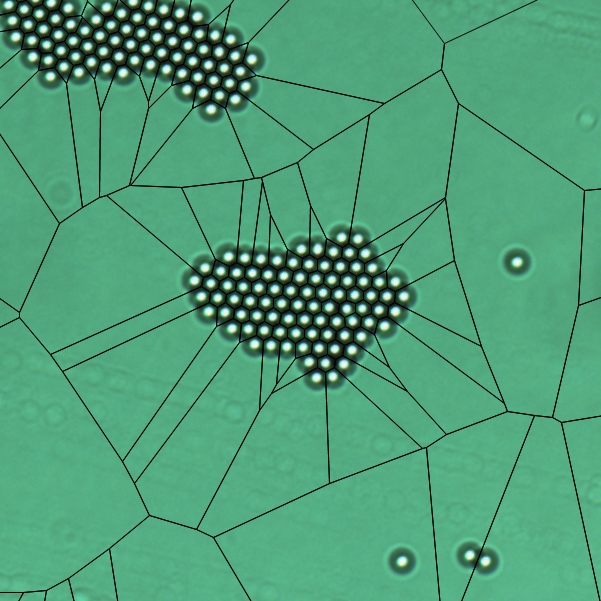
\includegraphics[width=\textwidth, keepaspectratio]{voronoiExp}}
\caption{\tiny Ячейки Вороного}
\end{figure}
\end{column}



\begin{column}{0.3\linewidth}
\begin{figure}[h]
\center{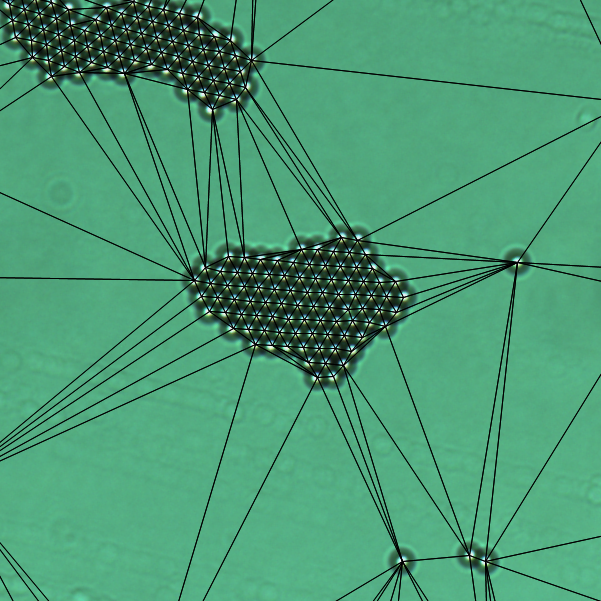
\includegraphics[width=\textwidth, keepaspectratio]{deluanau}}
\caption{\tiny Триангуляция Делоне}
\end{figure}
\end{column}



\begin{column}{0.3\linewidth}
\begin{figure}[h]
\center{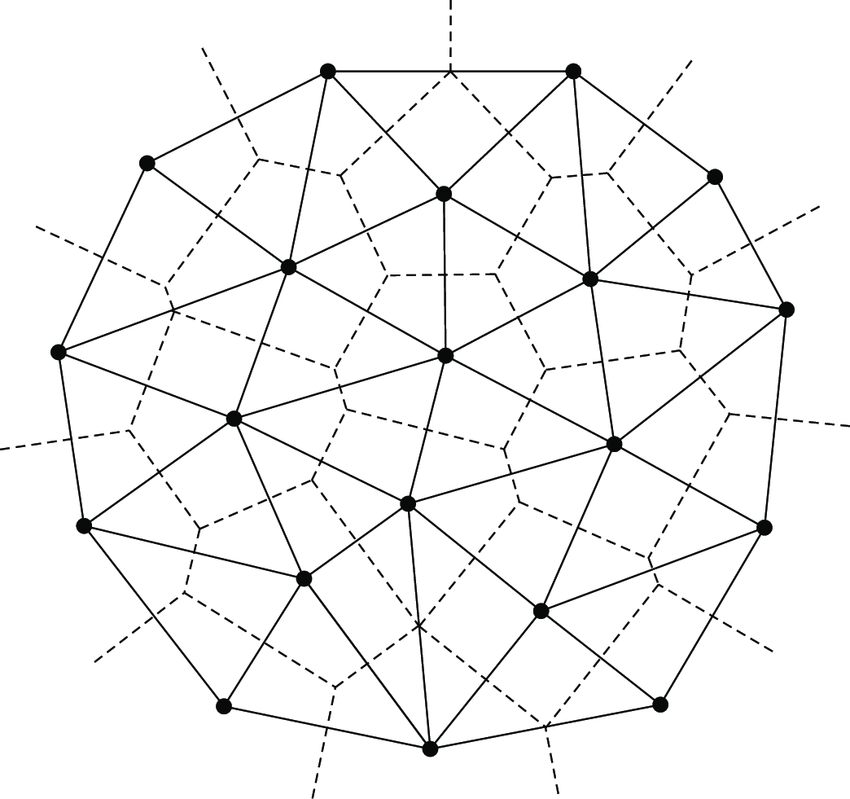
\includegraphics[width=\textwidth, keepaspectratio]{Delaunay-voron}}
\caption{\tiny Проведение перпендикуляров}
\end{figure}
\end{column}


\end{columns}

\vspace{17mm}
\tiny{
Ovcharov P. V. et al. Particle-resolved phase identification in two-dimensional condensable systems //The Journal of Physical Chemistry C. – 2017. – Т. 121. – №. 48. – С. 26860-26868.
}

\end{frame}



\begin{frame}%четвертый слайд
\transdissolve[duration=0.2]
\frametitle{Разбиение на ячейки Вороного}

\begin{columns}


\begin{column}{0.47\linewidth}
\begin{figure}[h]

\center{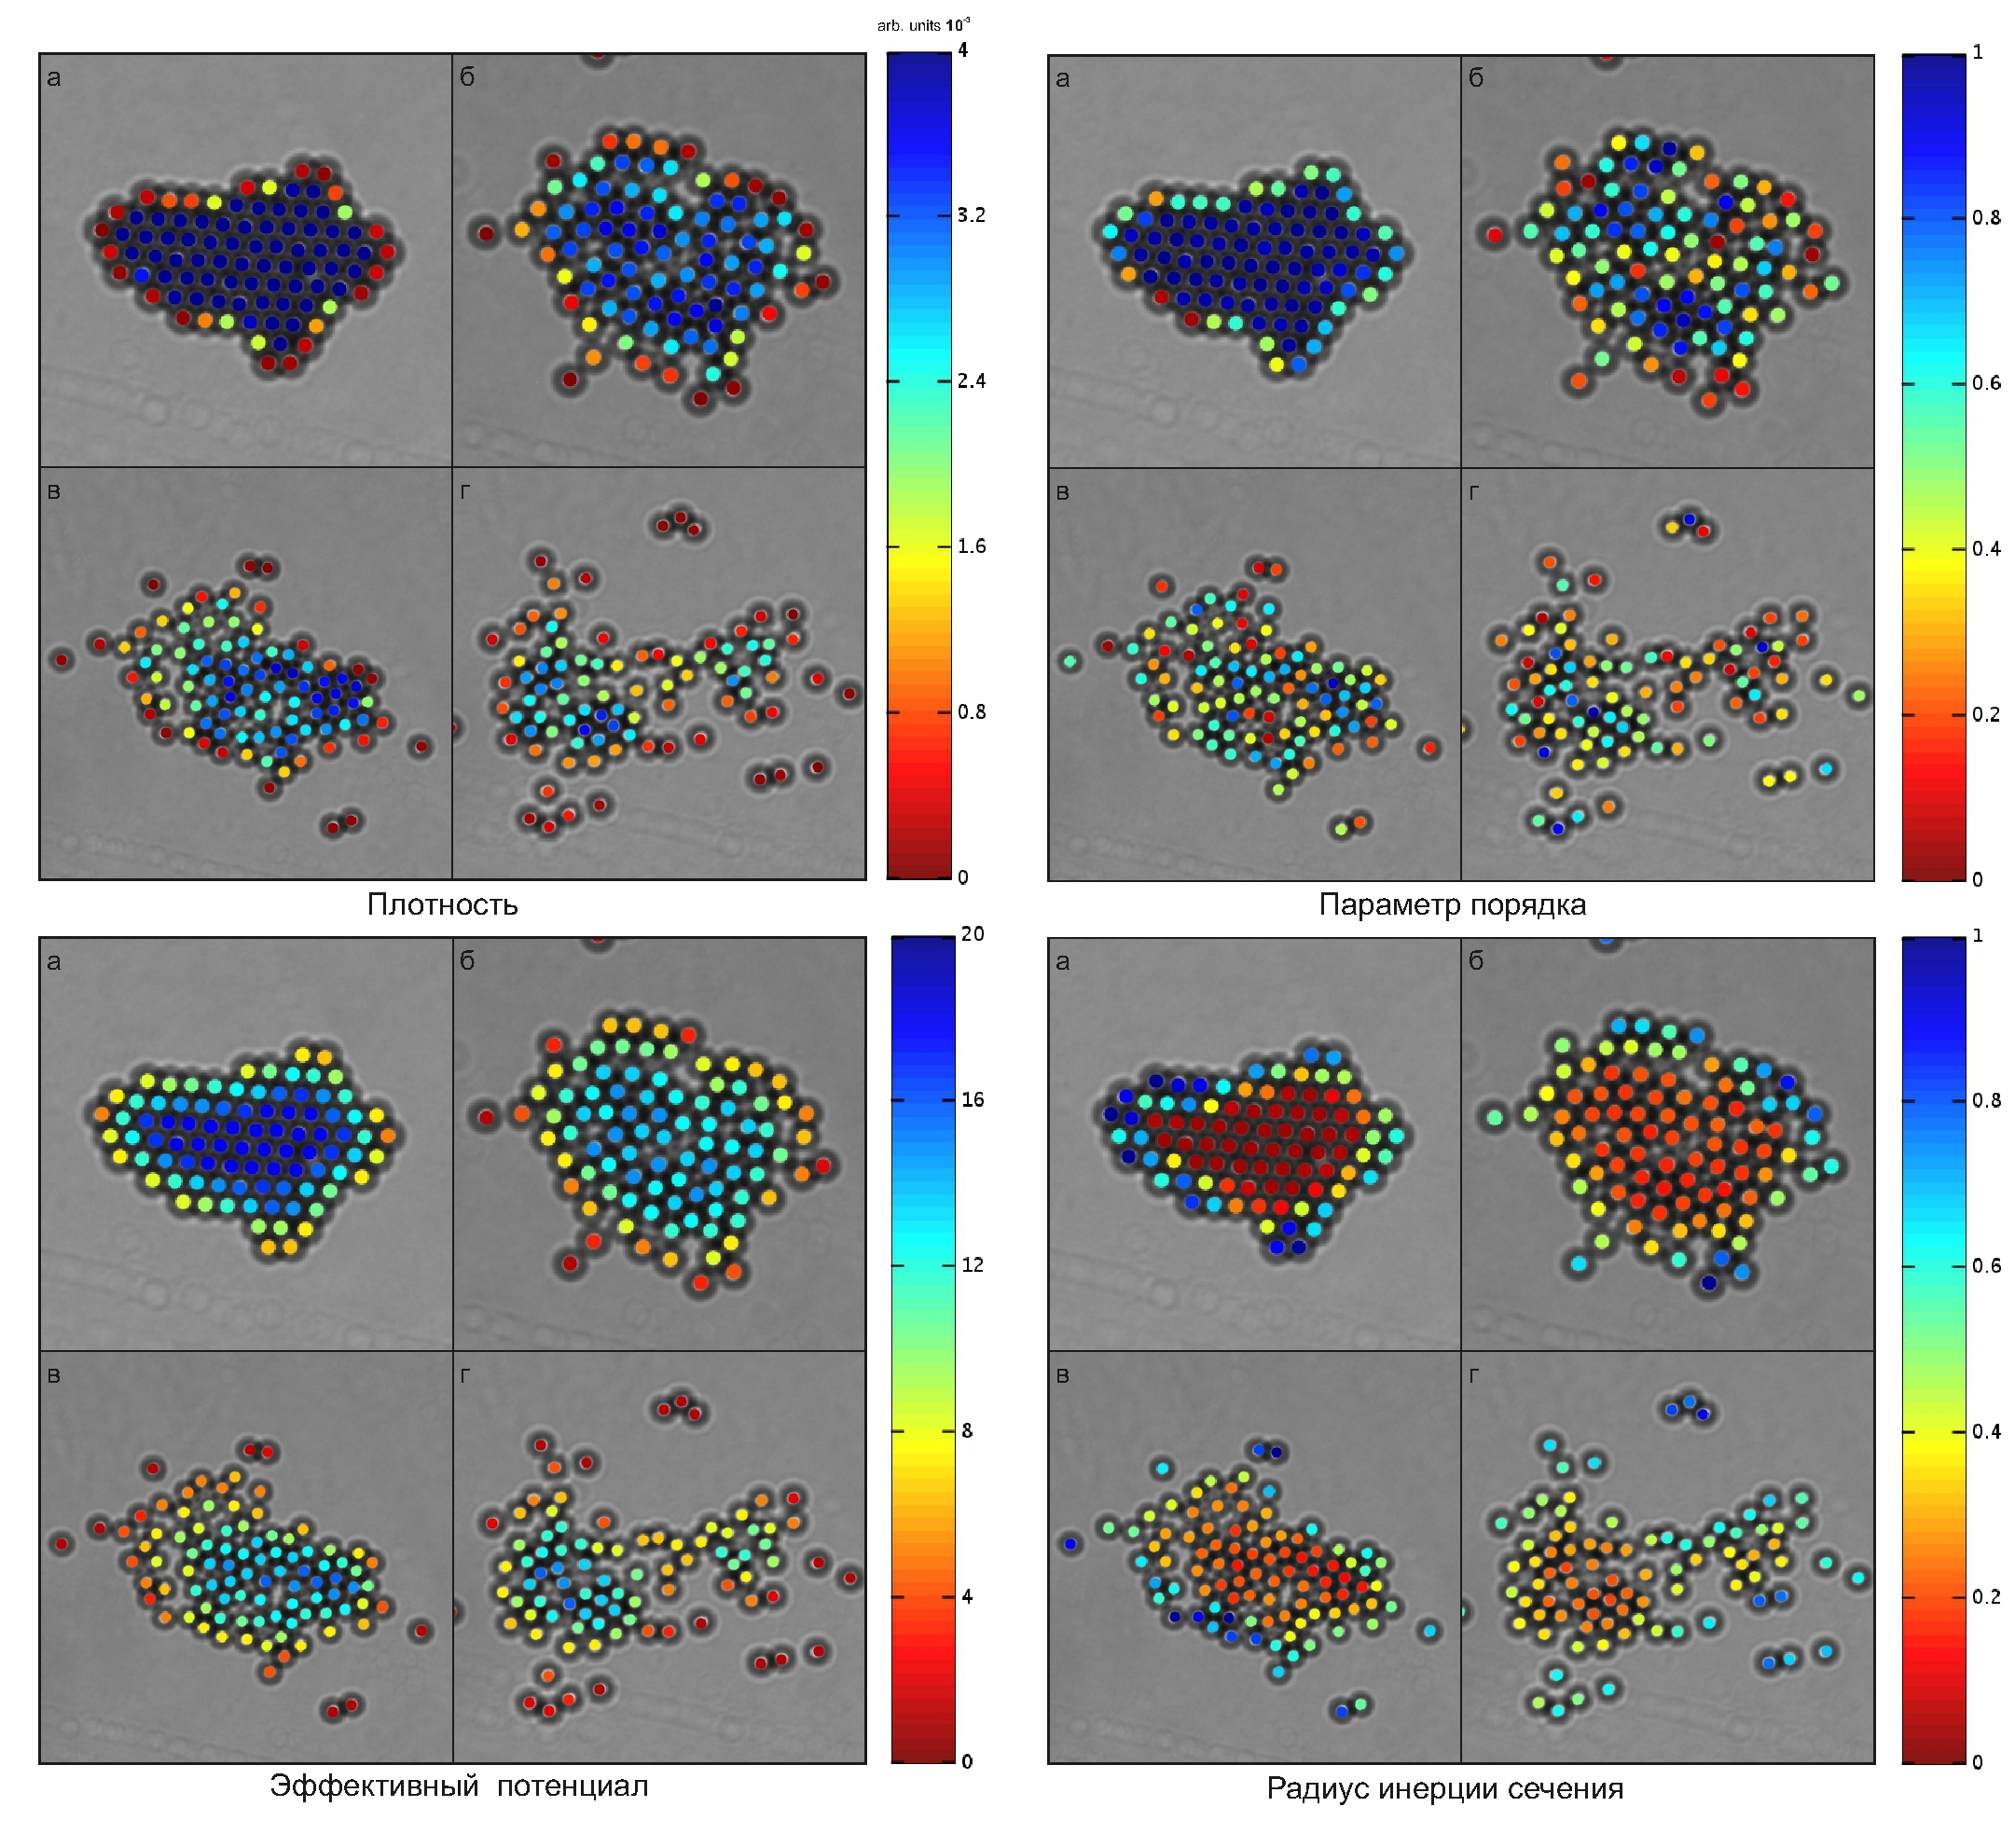
\includegraphics[width=\textwidth,  keepaspectratio]{PIVTURES}}
\caption{ \tiny Изображение различных параметров, посчитанных с помощью разбиения на ячейки Вороного (плотность, параметр порядка, эффективные потенциалы, радиусы инерции сечения).}
\end{figure}
\end{column}


\begin{column}{0.47\linewidth}

\tiny{
\begin{itemize}
\item Найти соседей каждой частицы
\item Плотности
\item Параметры порядка
\item Эффективные потенциалы
\item Радиусы инерции сечения
\item И т.д.
\end{itemize}
}
\end{column}


\end{columns}

\vspace{5mm}
\tiny{
Ovcharov P. V. et al. Particle-resolved phase identification in two-dimensional condensable systems //The Journal of Physical Chemistry C. – 2017. – Т. 121. – №. 48. – С. 26860-26868.
}
\end{frame}


\subsection{Метод распознавания фаз}


\begin{frame}%пятый слайд
\transdissolve[duration=0.2]
\frametitle{Параметр иррегулярности $R$}

\begin{columns}

\begin{column}{0.47\linewidth}

\begin{figure}[h]
\center{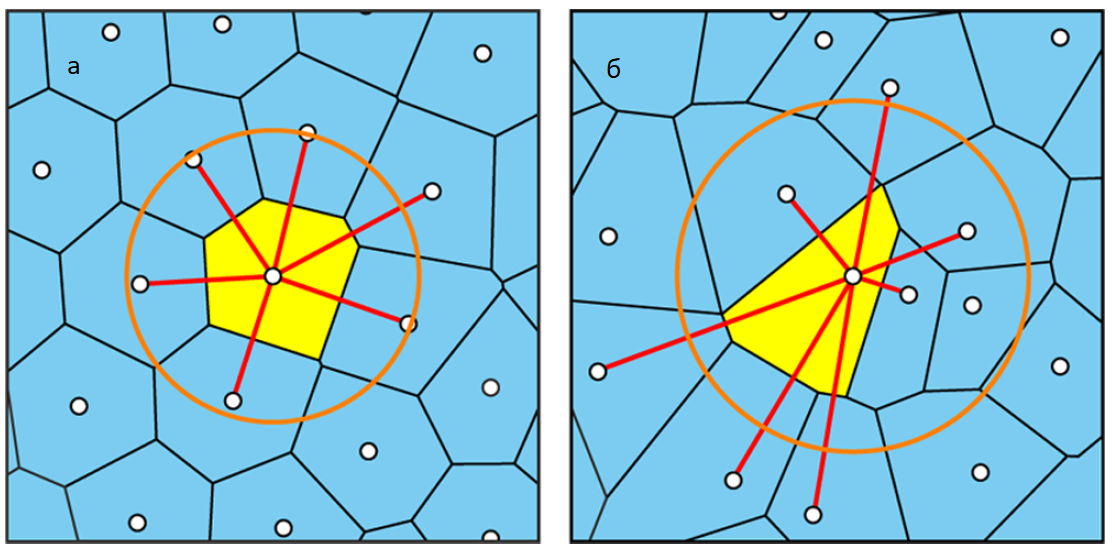
\includegraphics[width=0.7\textwidth, keepaspectratio]{rgcell}}
\caption{ \tiny а) Кристалл б) Газ.}
\end{figure}


\tiny{
\begin{equation}
\begin{aligned}
R_{0i} &= \sqrt{\frac{\pi}{2 S_i N_{ni}^2} \sum\limits_{i<k}^{N_{ni}} (r_{ij} - r_{ik})^2}, r_{ij} = |r_i - r_j| \\
R_i &= \frac{1}{N_{ni} + 1} \left( R_{0i} + \sum\limits_{j=1}^{N_{ni}} R_{0j} \right)
\end{aligned}
\label{eqR}
\end{equation}
}
\tiny{где $S_i$ - площадь ячейки, $N_{ni}$ - количество соседей, $r_{ij}$ - расстояние от рассматриваемой частицы до соседней.}


\end{column}
\begin{column}{0.47\linewidth}

\begin{figure}[h]
\center{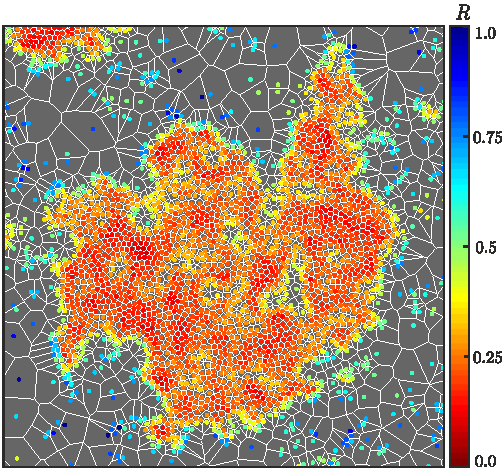
\includegraphics[width=\textwidth,  keepaspectratio]{MPI-Figure1}}
\caption{ \tiny Распределение параметра $R$.}
\end{figure}

\end{column}
\end{columns}
\vspace{3mm}
\tiny{
Ovcharov P. V. et al. Particle-resolved phase identification in two-dimensional condensable systems //The Journal of Physical Chemistry C. – 2017. – Т. 121. – №. 48. – С. 26860-26868.
}
\end{frame}




\begin{frame}
\transdissolve[duration=0.2]
\frametitle{Корректировка фаз}
\begin{columns}

\begin{column}{0.47\linewidth}

\begin{figure}[h]
\center{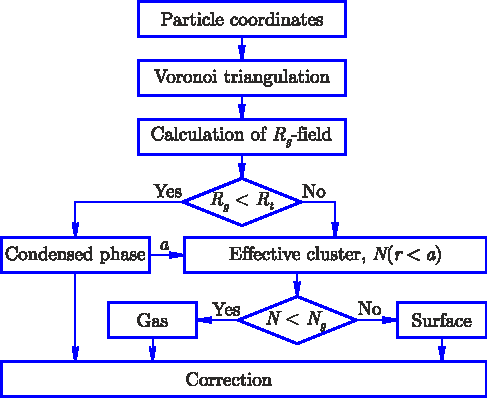
\includegraphics[width=\textwidth,  keepaspectratio]{PRM-Figure1-eps-converted-to}}
\caption{\tiny Алгоритм классификации частиц в системе.}
\end{figure}

\end{column}

\begin{column}{0.47\linewidth}
\tiny{
Корректировка фаз включает в себя следующие условия:
\begin{itemize}
\item частица конденсата, не имеющая среди своих соседей частиц того же типа, является поверхностью.
\item частица конденсата, которая имеет среди соседних частиц, газовую частицу, является поверхностью.
\item газовая частица, не имеющая соседних частиц того же класса,  является поверхностью.
\item частица поверхности, все соседи которой принадлежат к классу "конденсат" или "газ", так же принадлежат к этому классу.
\end{itemize}
}
\end{column}

\end{columns}

\vspace{12mm}
\tiny{
Ovcharov P. V. et al. Particle-resolved phase identification in two-dimensional condensable systems //The Journal of Physical Chemistry C. – 2017. – Т. 121. – №. 48. – С. 26860-26868.
}
\end{frame}





\begin{frame}
\transdissolve[duration=0.2]
\frametitle{Недостатки метода распознавания фаз}

\begin{columns}

\begin{column}{0.47\linewidth}

\begin{figure}[h]
\center{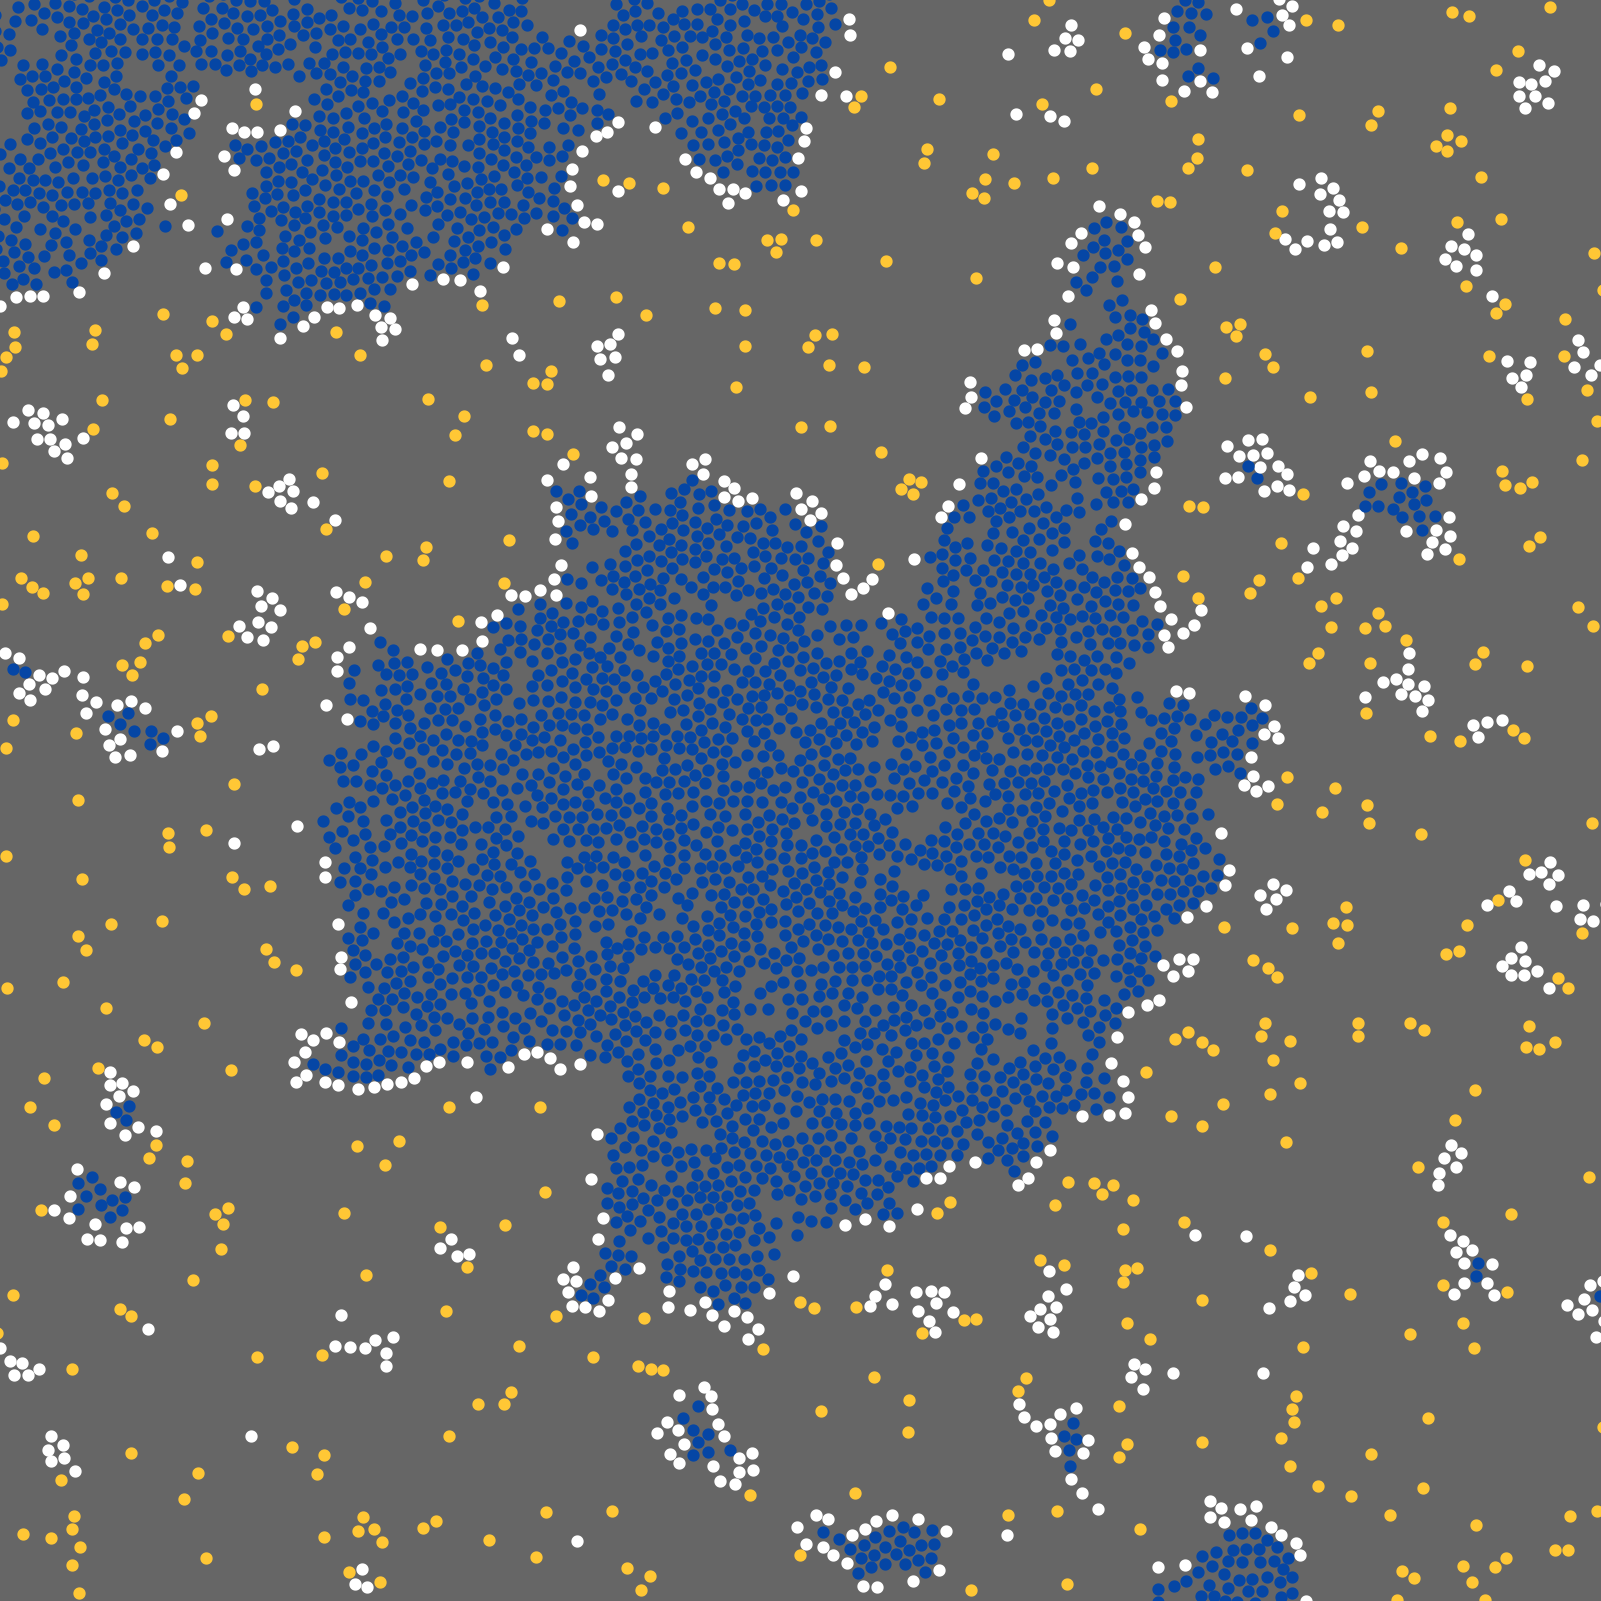
\includegraphics[width=\textwidth,  keepaspectratio]{phas_200_0.48_cut}}
\caption{\tiny Результат алгоритма классификации.}
\end{figure}

\end{column}


\begin{column}{0.47\linewidth}
\tiny{
Недостатки метода распознавания фаз:
\begin{itemize}
\item распознавание пустот внутри конденсированного кластера, как его часть.
\item скопления поверхностных частиц, которые могут быть небольшими кластерами.
\item нерегулярная граница кластера из поверхностных частиц.
\item частицы на поверхности кластера с низкой плотностью, распознанные как конденсат а не поверхность, вносят ошибку в вычисления мат. ожидания плотности.
\end{itemize}
}
\end{column}

\end{columns}

\vspace{5mm}
\tiny{
Ovcharov P. V. et al. Particle-resolved phase identification in two-dimensional condensable systems //The Journal of Physical Chemistry C. – 2017. – Т. 121. – №. 48. – С. 26860-26868.
}

\end{frame}




\begin{frame}
\transdissolve[duration=0.2]
\frametitle{Изменения в корректировке фаз}

\begin{columns}

\begin{column}{0.47\linewidth}
\tiny{
Дополнительные условия в корректировки фаз:
\begin{itemize}
\item частица поверхности, не имеющая среди соседей частиц газа, является конденсатом.
\item поверхностная частица, не имеющая среди соседей частиц конденсата, является газом.
\item частицы конденсата, плотность которых сопоставима с плотностью поверхностных частиц, являются поверхностью. Данная проверка делается дважды (перед всеми остальными и после).
\item частица конденсата, которая имеет меньше 3 соседних частиц, так же принадлежащих к конденсату, является поверхностью.
\end{itemize}
}
\end{column}


\begin{column}{0.47\linewidth}

\begin{figure}[h]
\center{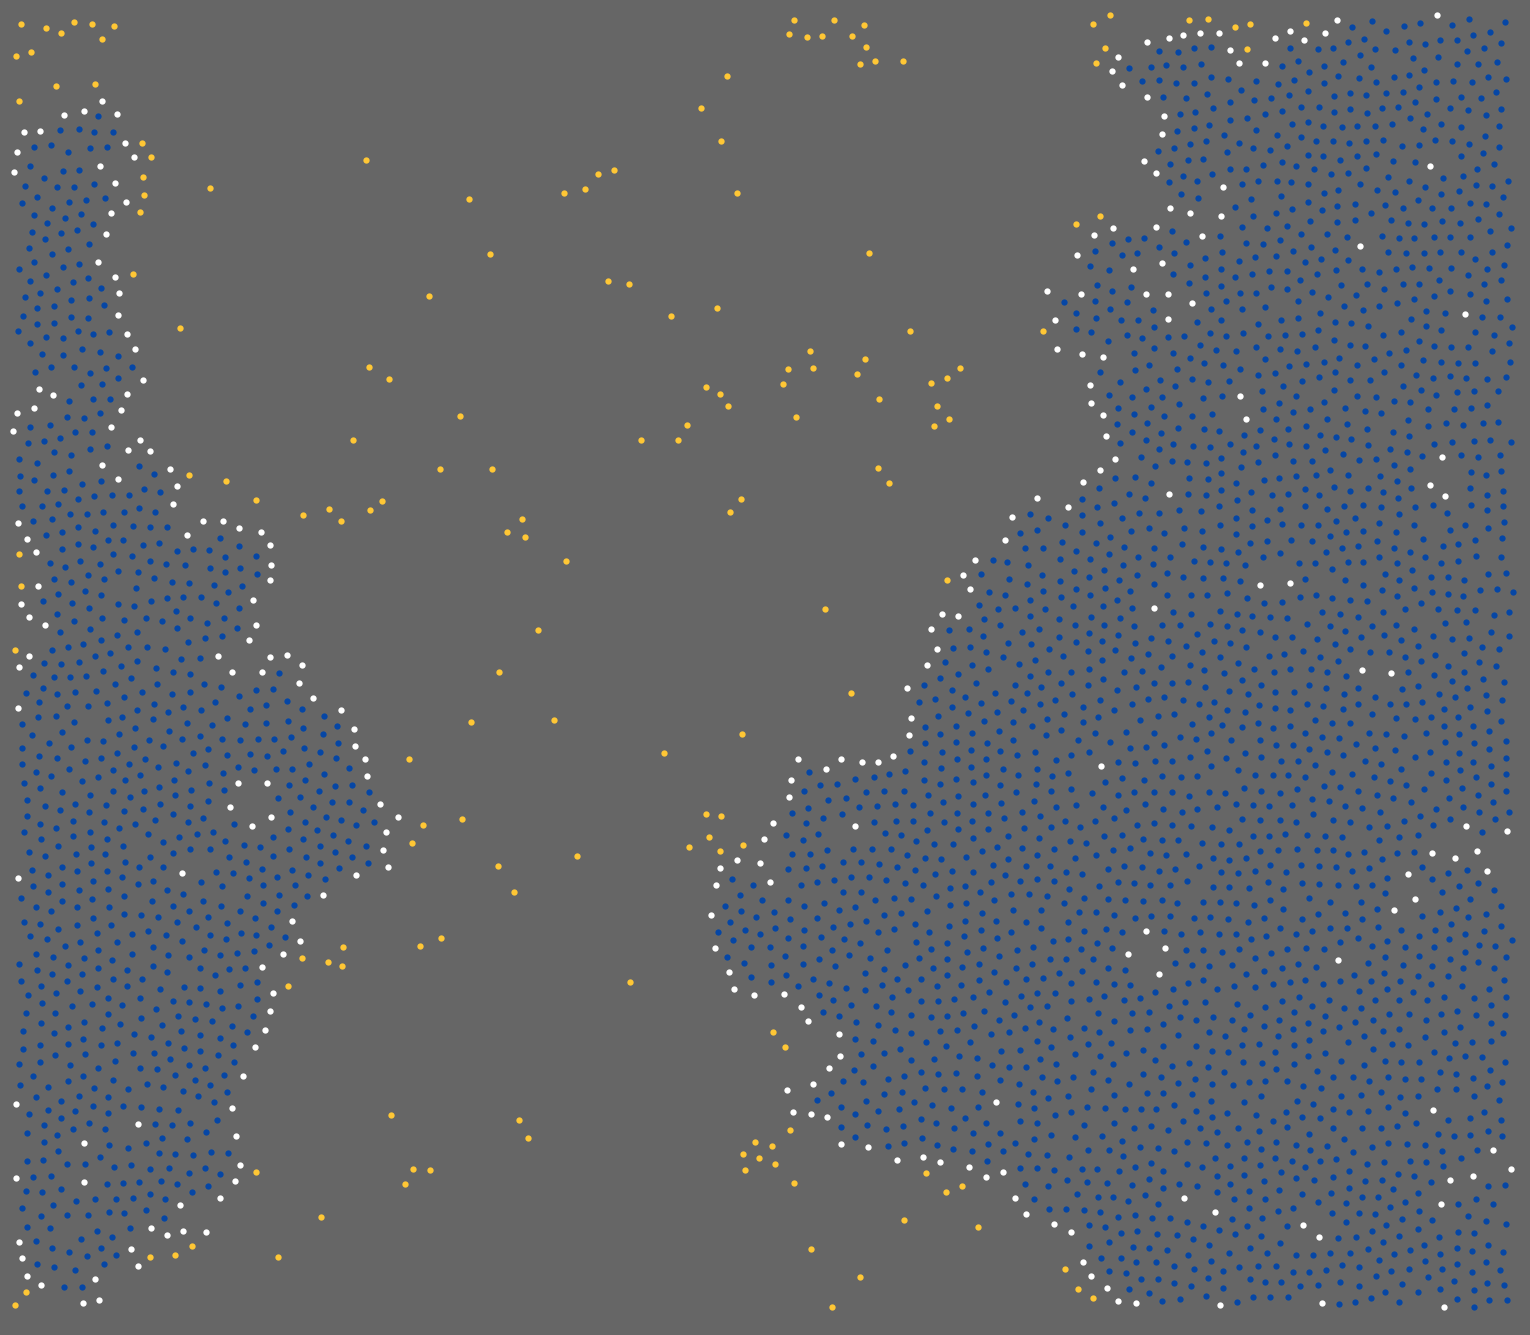
\includegraphics[width=\textwidth,  keepaspectratio]{phas_2}}
\caption{\tiny Результат обновленного алгоритма классификации.}
\end{figure}

\end{column}

\end{columns}

\end{frame}





\subsection{Построение фазовой диаграммы}


\begin{frame}
\transdissolve[duration=0.2]
\frametitle{Нахождение точек на фазовой диаграмме}
\begin{columns}


\begin{column}{0.55\linewidth}

\begin{figure}[h]
\center{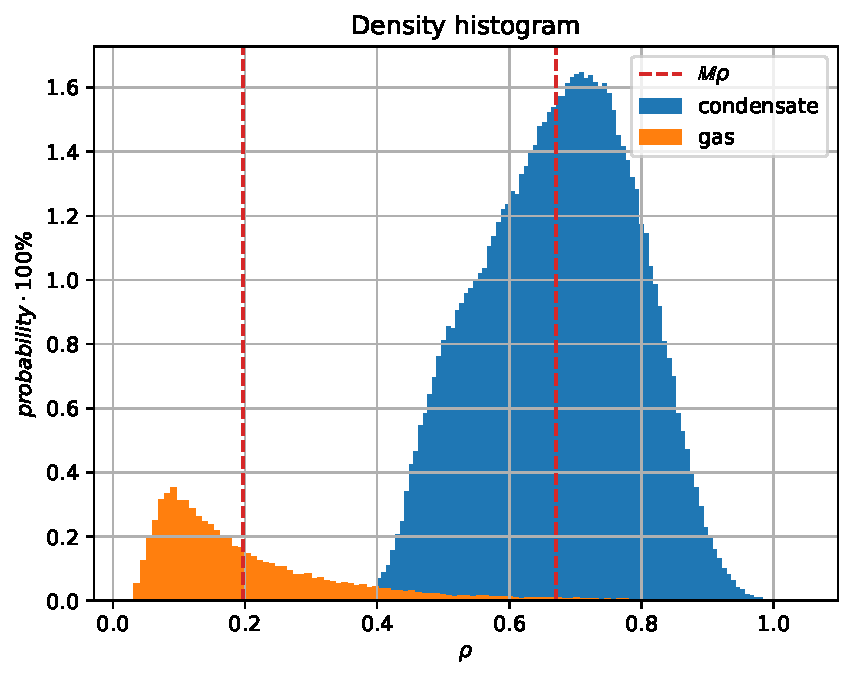
\includegraphics[width=\textwidth,  keepaspectratio]{Mrho}}
\end{figure}

\end{column}

\begin{column}{0.4\linewidth}

\begin{figure}[h]
\center{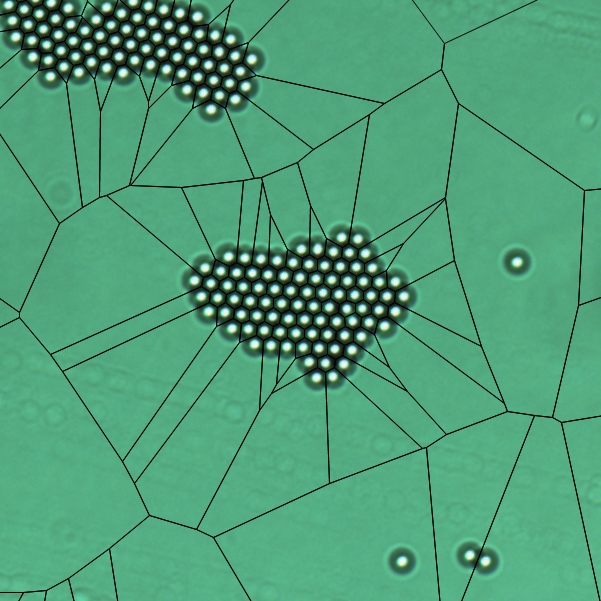
\includegraphics[width=\textwidth,  keepaspectratio]{voronoiExp}}
\end{figure}

\end{column}

\end{columns}

\vspace{15mm}
\tiny{
Ovcharov P. V. et al. Particle-resolved phase identification in two-dimensional condensable systems //The Journal of Physical Chemistry C. – 2017. – Т. 121. – №. 48. – С. 26860-26868.
}
\end{frame}




\begin{frame}
\transdissolve[duration=0.2]
\frametitle{Изменения в определении плотности газа}
\begin{columns}


\begin{column}{0.55\linewidth}

\begin{figure}[h]
\center{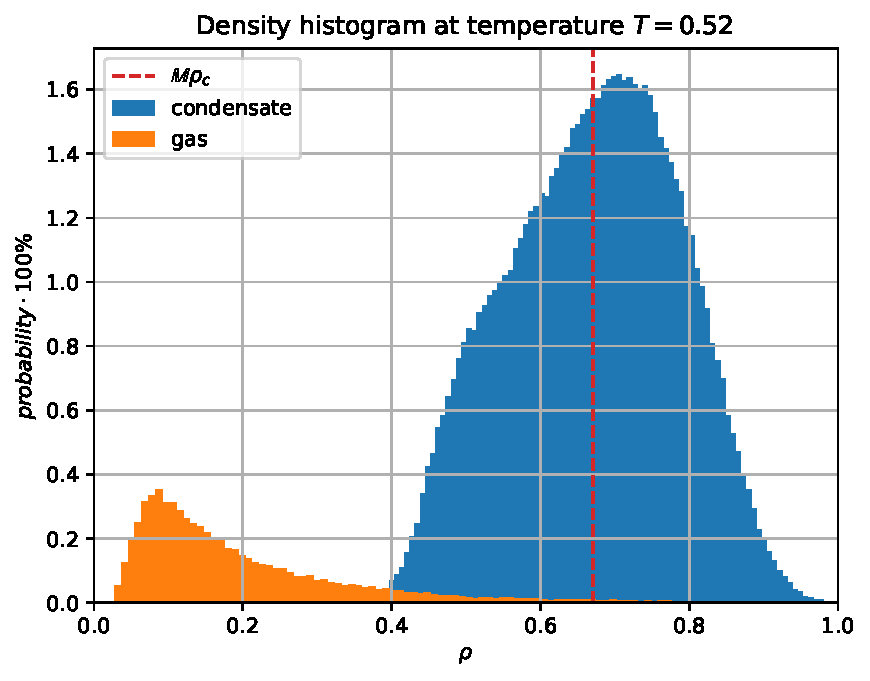
\includegraphics[width=\textwidth,  keepaspectratio]{plot_hist_all_0.520}}
\end{figure}

\end{column}

\begin{column}{0.4\linewidth}

\tiny{
Плотность газа в системе вычисляется косвенно по формуле:
\begin{equation}
\rho_{gas} = \frac{N_{g}}{S - (N_{b} + N_{c}) / \mathbb{M}\rho_c},
\label{eqGas}
\end{equation}
где $S$ - суммарная площадь всех рассматриваемых кадров, $N_g, N_b, N_c$ - суммарное число частиц газа, поверхности и конденсата соответственно на всех рассматриваемых кадрах моделирования, $\mathbb{M}\rho_c$ - мат. ожидание плотности частиц конденсата на всех рассматриваемых кадрах.
}

\end{column}

\end{columns}
\end{frame}


%\section{Результаты анализа распределений}

\subsection{Построение фазовых диаграмм для различных потенциалов взаимодействия}

\begin{frame}
\begin{center}
\vspace{5mm}
\textbf{РЕЗУЛЬТАТЫ КВАЛИФИКАЦИОННОЙ РАБОТЫ}
\end{center}
\end{frame}







\begin{frame}
\transdissolve[duration=0.2]
\frametitle{Описание смоделированных систем}

\begin{columns}

\begin{column}{0.5\linewidth}

\begin{figure}[h]

\center{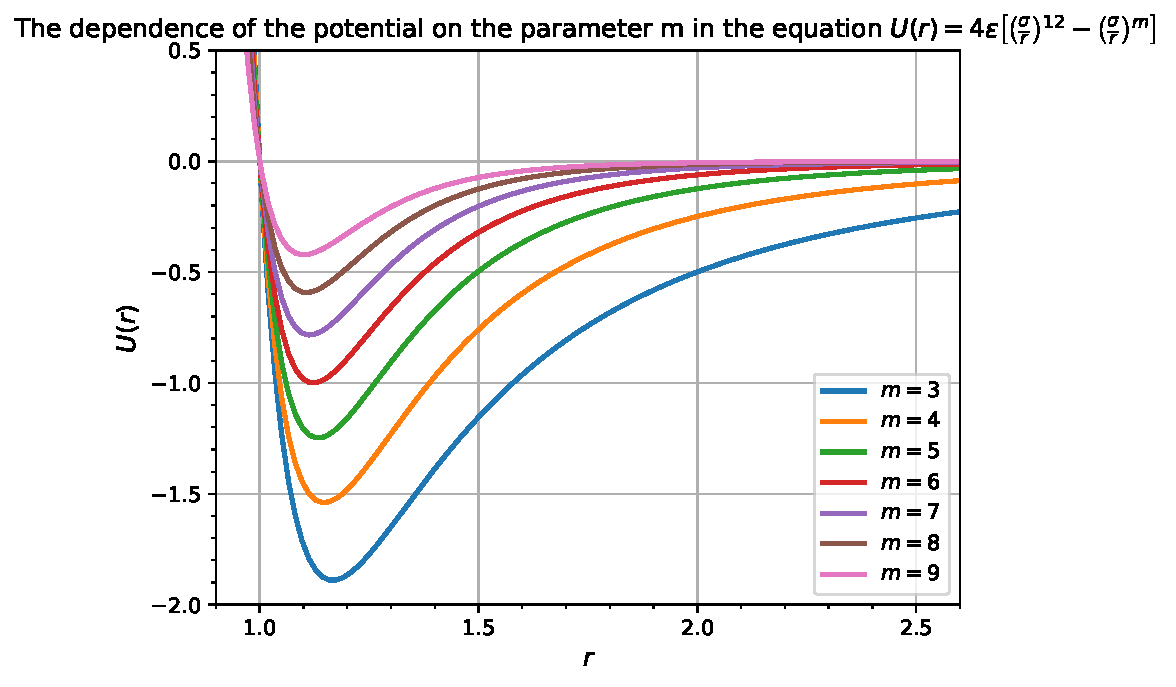
\includegraphics[width=\textwidth,  keepaspectratio]{LJ}}
\caption{\tiny Обобщенный потенциал Леннарда - Джонса с различными степенями притяжения.}
\end{figure}

\end{column}

\begin{column}{0.5\linewidth}
\tiny{

\begin{equation}
U(r) = 4\varepsilon \left[ \left(\frac{\sigma}{r}\right)^{12} - \left(\frac{\sigma}{r}\right)^{m} \right], m = 3, 4, 5, 6, 7, 8, 9.
\label{eqLJ}
\end{equation}

Каждое моделирование проводилось при постоянной температуре и плотности. Статистика собрана по 150 кадрам моделирования, на каждом из которых примерно по 3600 частиц. Все величины на графиках являются обезразмеренными с помощью $\varepsilon = 1, \sigma = 1, m = 1, k_B = 1$.

\begin{table}[H]
\begin{center}
\begin{tabular}{| l | l | l | l | l |}
\hline
    & LJ12-3 & LJ12-4 & LJ12-5 & LJ12-6 \\ \hline
$m$   &    3    &     4   &    5    &    6    \\ \hline
$\Delta T$ & 0.03 & 0.03 & 0.02 & 0.02 \\ \hline
$\rho_0$ & 0.3  &  0.4  &  0.4  &  0.4  \\ \hline
\end{tabular}
\end{center}
\caption{\tiny Параметры некоторых моделирований исследуемых систем. $m$ - степень слагаемого в уравнении \ref{eqLJ}, $\Delta T$ - шаг по температуре,  $\rho_0$ - плотность системы в целом.}
\label{tablParam}
\end{table}

}
\end{column}

\end{columns}
\end{frame}





\begin{frame}
\transdissolve[duration=0.2]
\frametitle{Применение метода ячеек Вороного}
\begin{columns}


\begin{column}{0.5\linewidth}

\begin{figure}[h]
\begin{center}
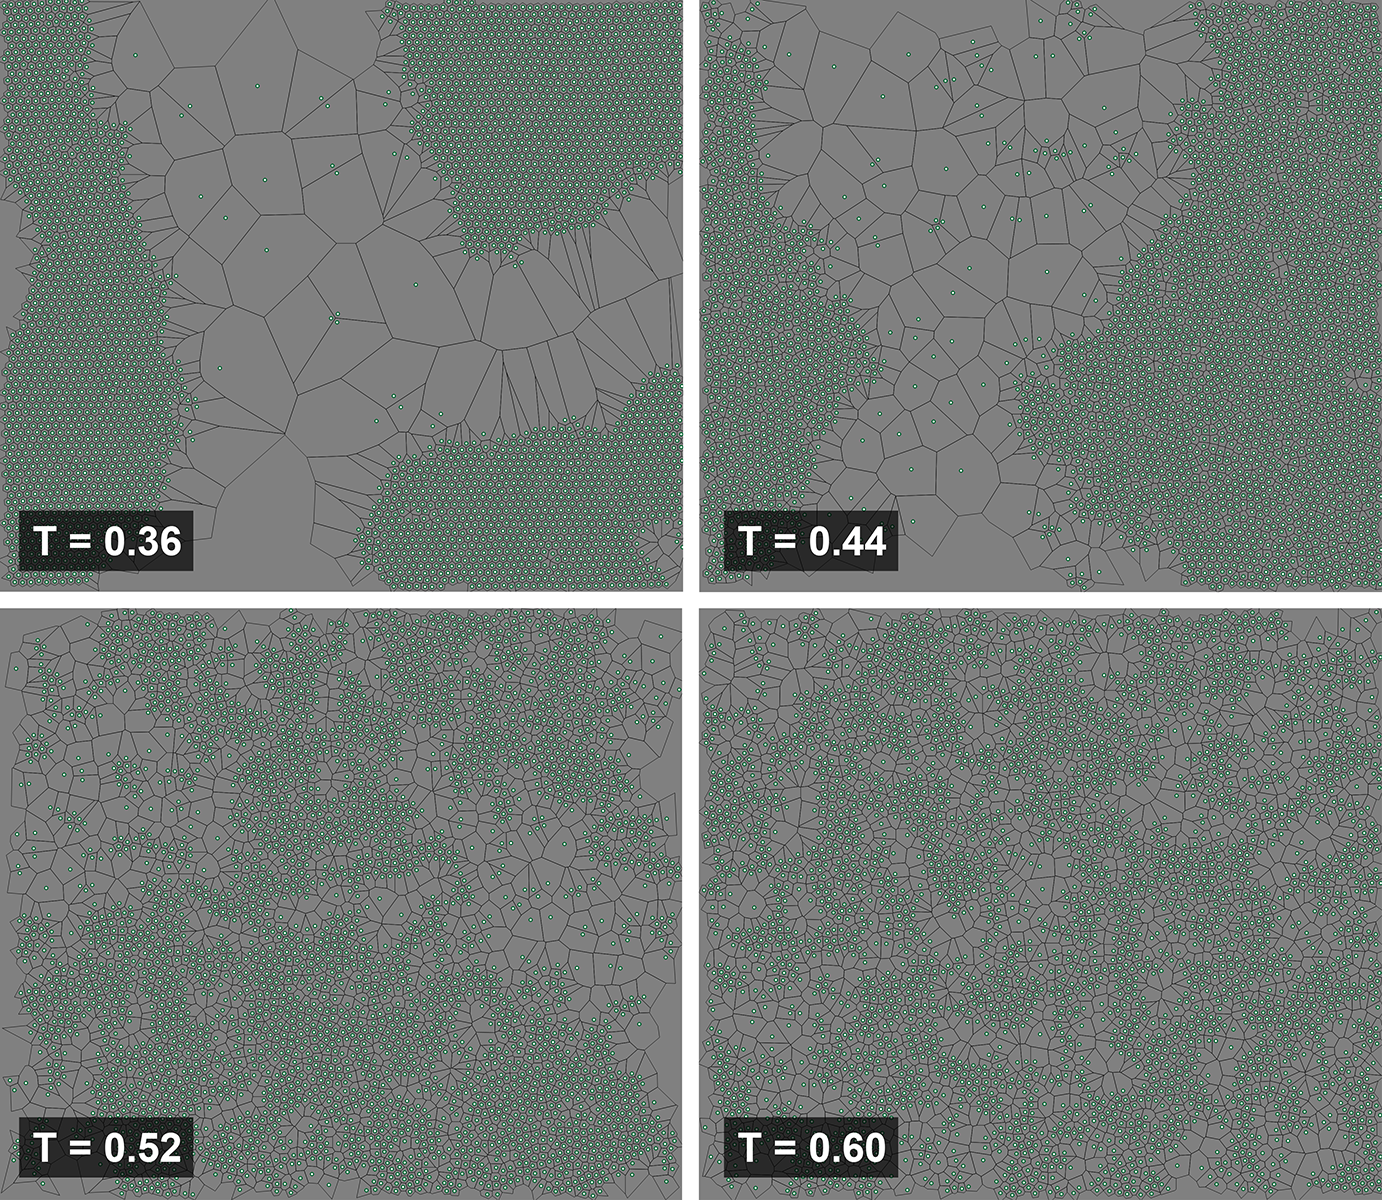
\includegraphics[width=\textwidth]{Voronoi}
\caption{\tiny Разбиение на ячейки Вороного различной температуре исследуемой в данной работе системы на примере потенциала Леннарда-Джонса.}
\label{risvoronoiExp}
\end{center}
\end{figure}

\end{column}

\begin{column}{0.55\linewidth}

\begin{figure}[h]
\begin{center}
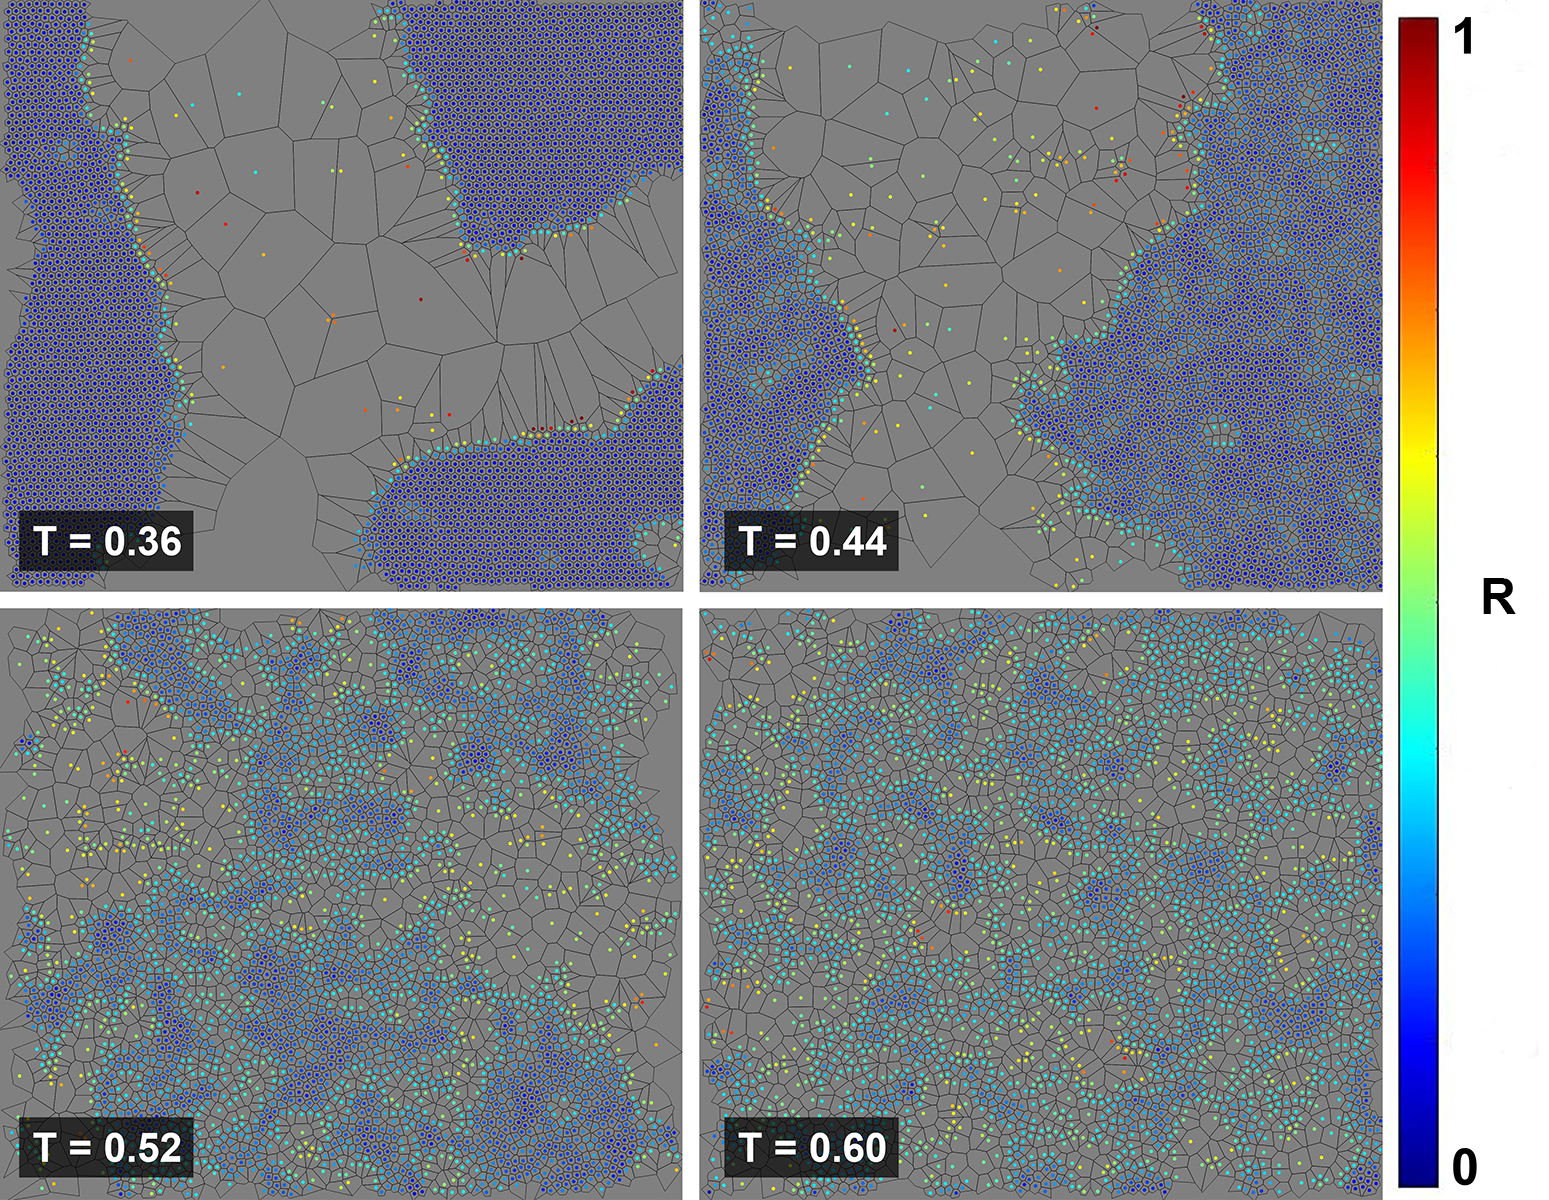
\includegraphics[width=\textwidth]{RG}
\caption{\tiny Параметр иррегулярности $R$ в исследуемой системе, на примере потенциала взаимодействия Леннарда-Джонса при различной температуре.}
\label{risIregExp}
\end{center}
\end{figure}

\end{column}

\end{columns}
\end{frame}





\begin{frame}
\transdissolve[duration=0.2]
\begin{columns}


\begin{column}{0.45\linewidth}

\begin{figure}[h]
\begin{center}
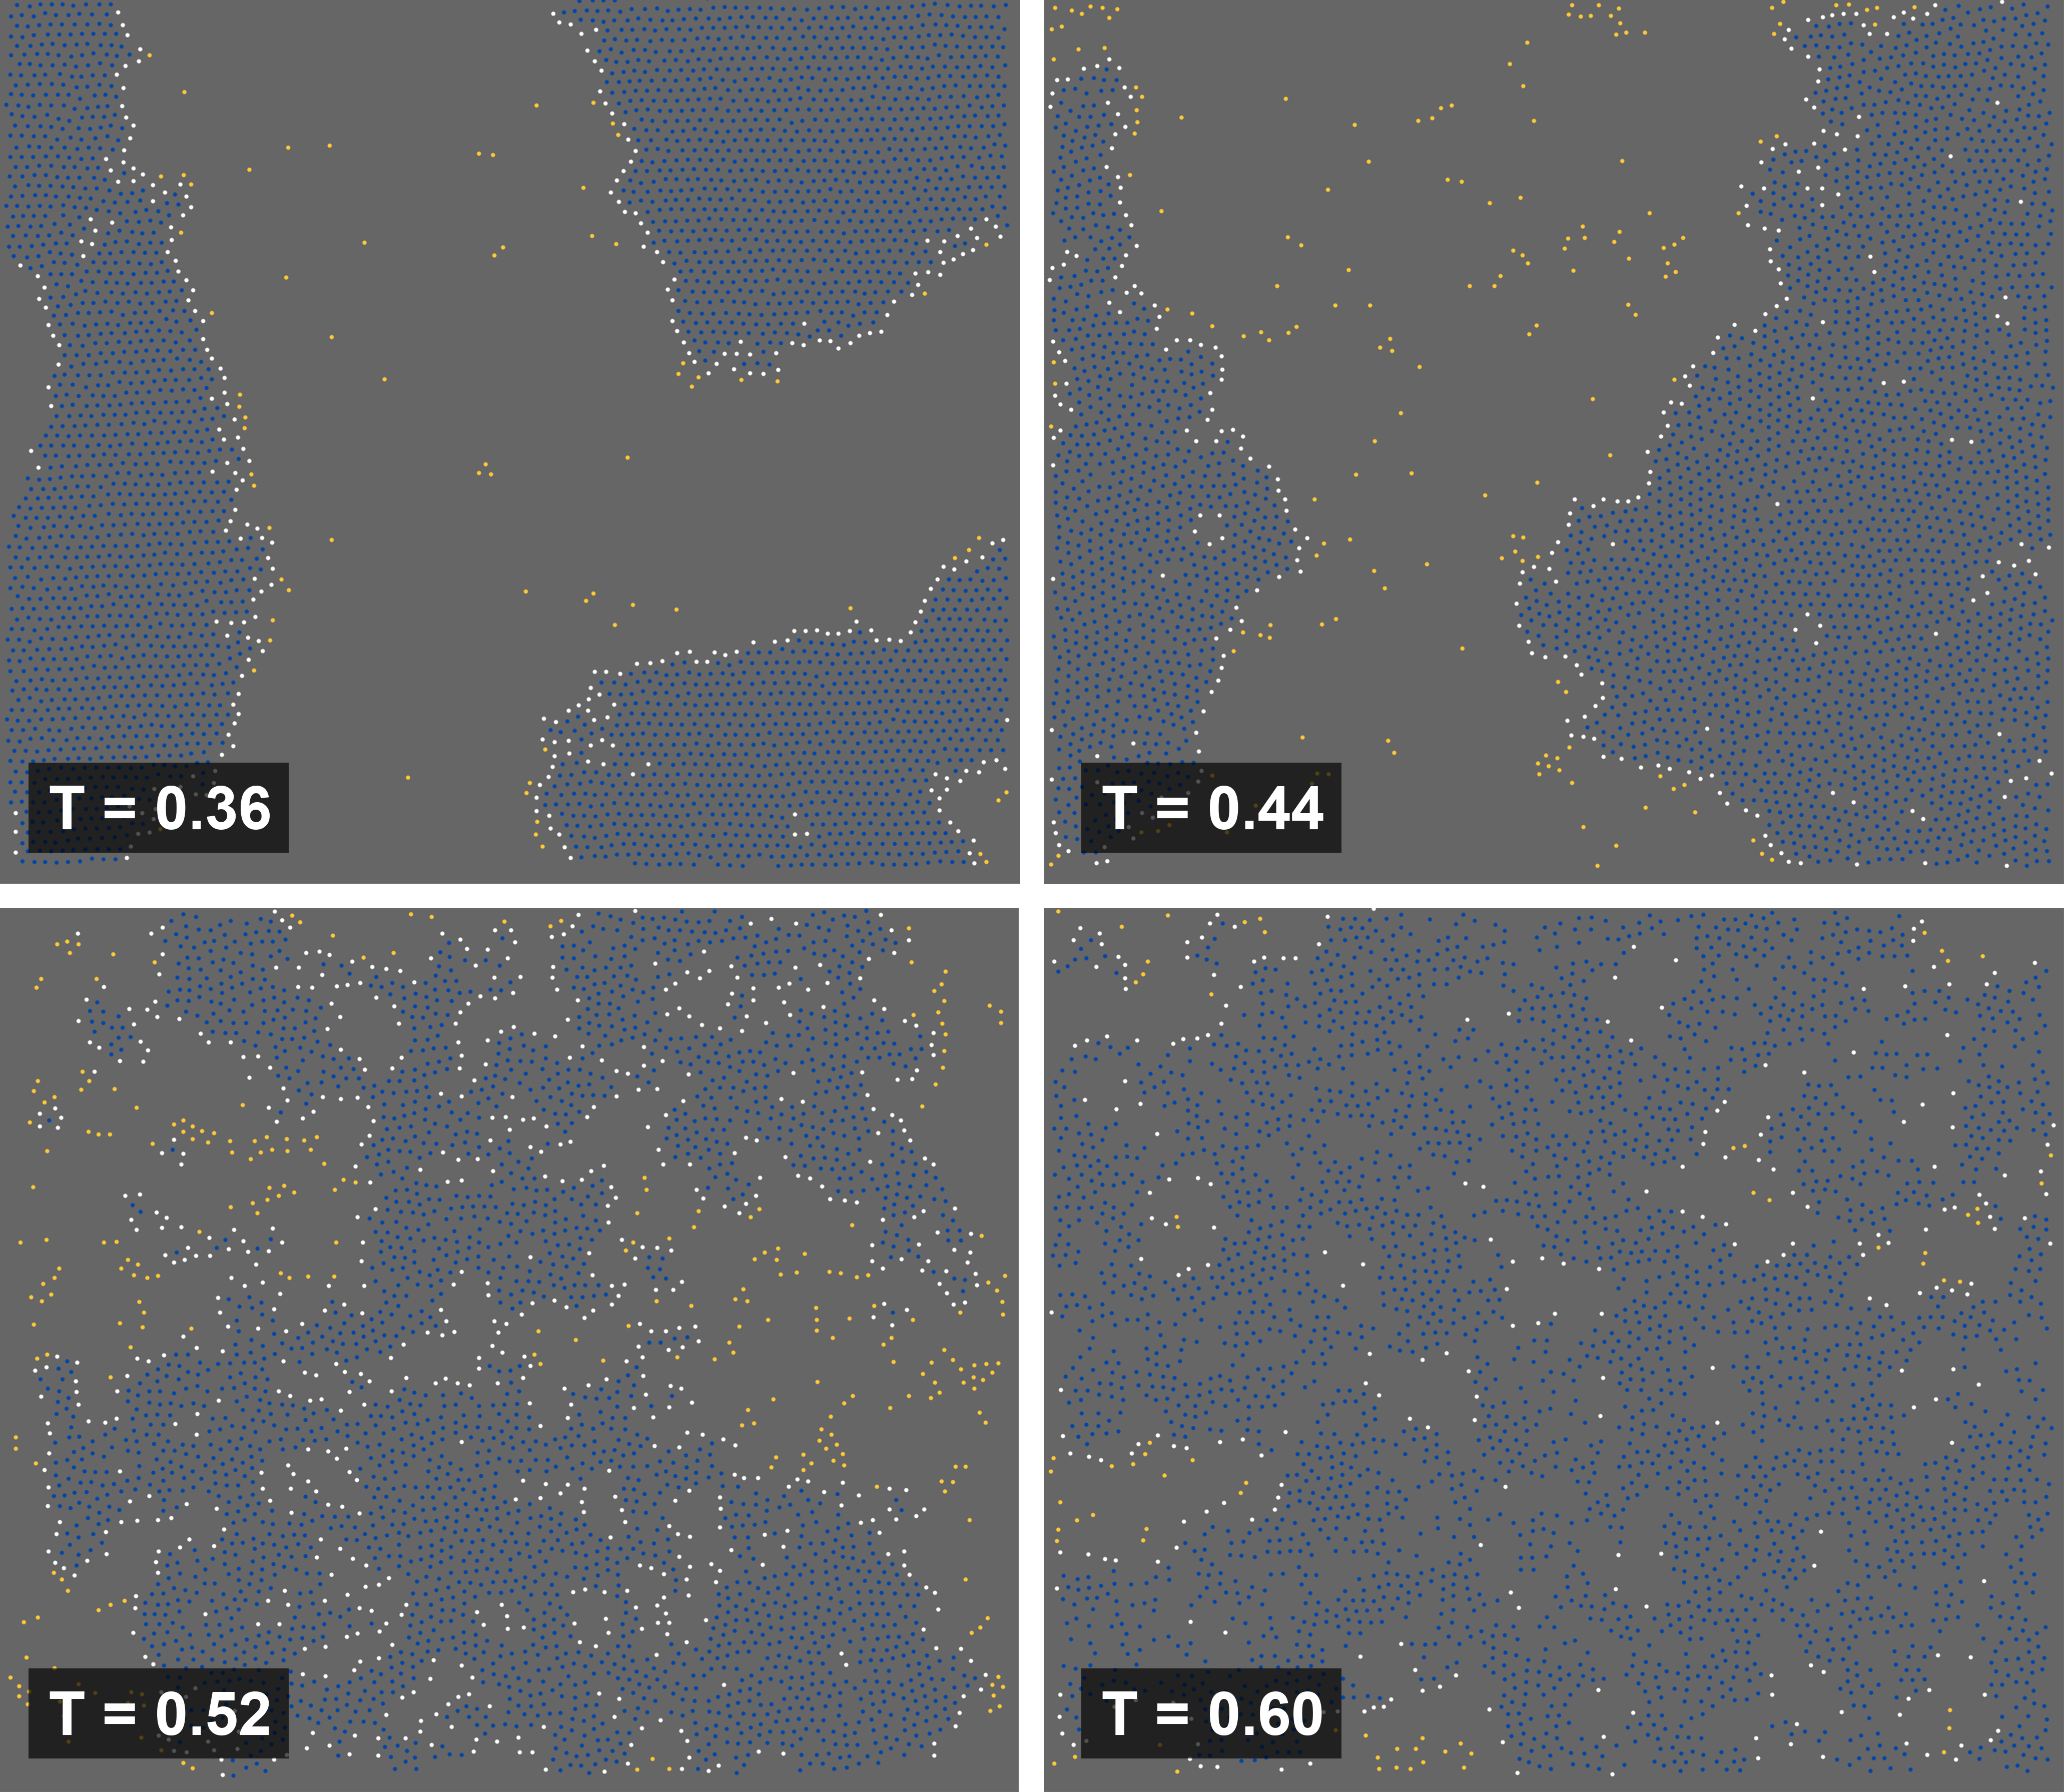
\includegraphics[width=\textwidth]{classification}
\caption{\tiny Классификация частиц в исследуемой системы на примере системы c потенциалом взаимодействия Леннарда-Джонса при различной температуре.}
\label{risClassExp}
\end{center}
\end{figure}

\end{column}

\begin{column}{0.55\linewidth}

\begin{figure}[h]
\begin{center}

\begin{minipage}[h]{0.47\linewidth}
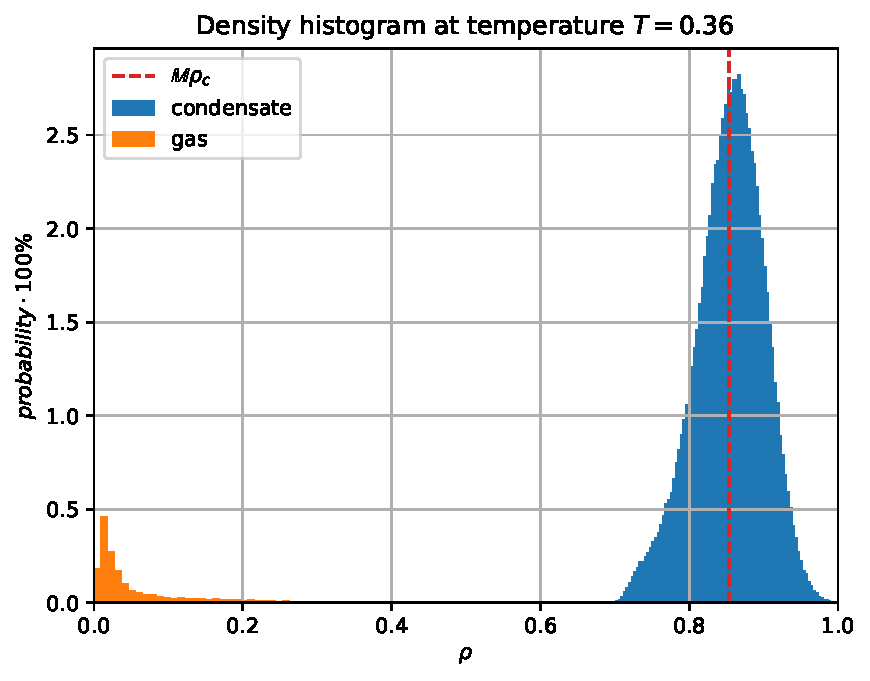
\includegraphics[width=\textwidth, keepaspectratio]{plot_hist_all_0.360}
\end{minipage}
%\hfill
\begin{minipage}[h]{0.47\linewidth}
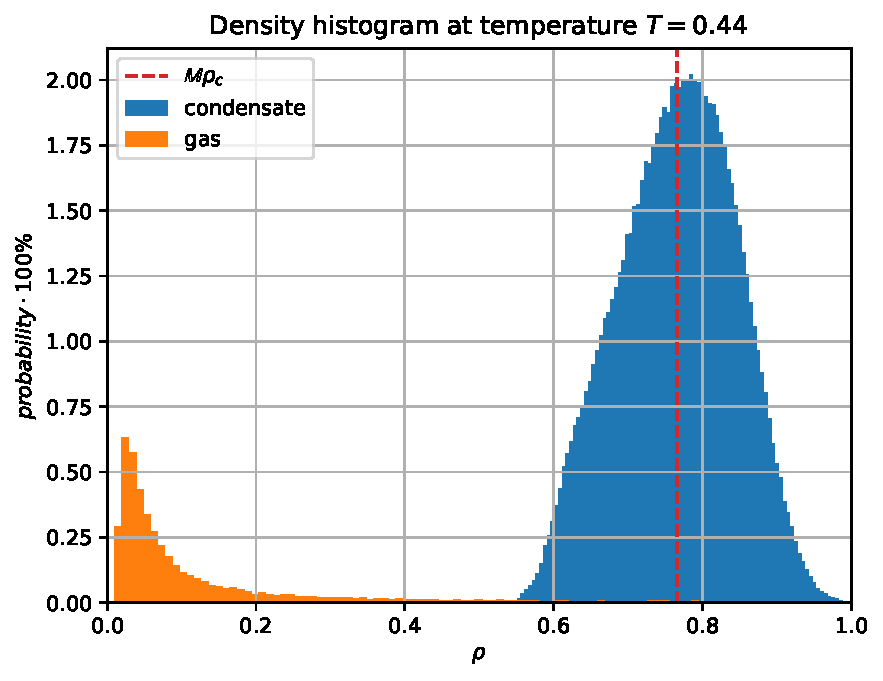
\includegraphics[width=\textwidth, keepaspectratio]{plot_hist_all_0.440}
\end{minipage}

\begin{minipage}[h]{0.47\linewidth}
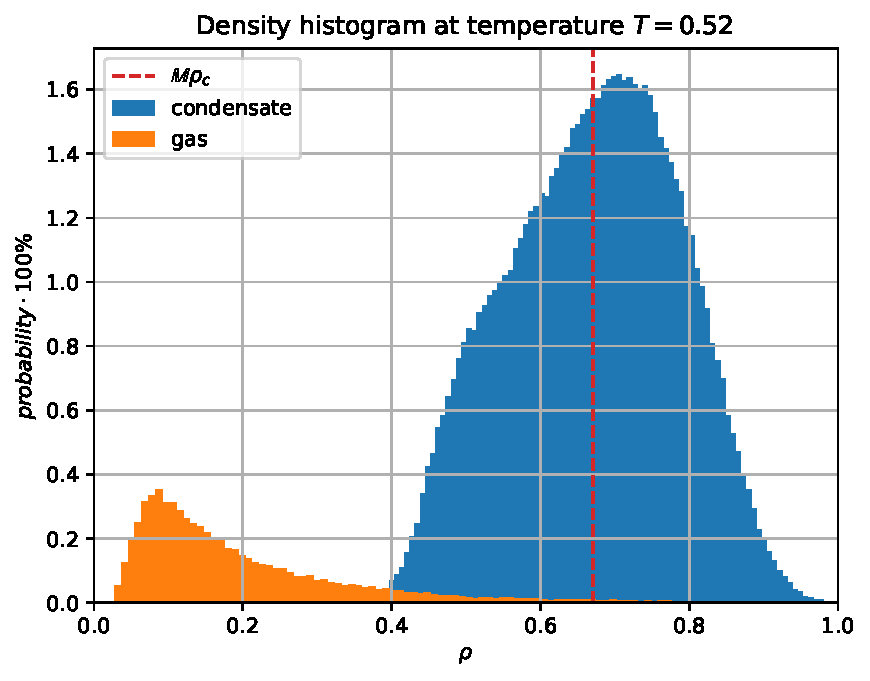
\includegraphics[width=\textwidth, keepaspectratio]{plot_hist_all_0.520}
\end{minipage}
%\hfill
\begin{minipage}[h]{0.47\linewidth}
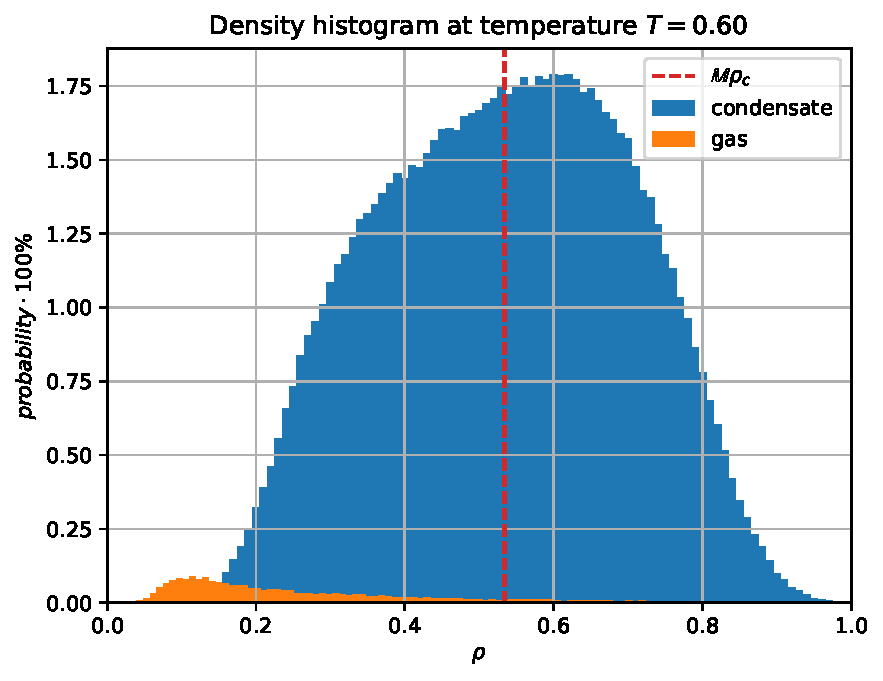
\includegraphics[width=\textwidth, keepaspectratio]{plot_hist_all_0.600}
\end{minipage}
\caption{\tiny Распределение плотностей частиц конденсата и газа при различных температурах. Синим цветом обозначен конденсат, оранжевым  - газ.}
\label{risRhoM}
\end{center}
\end{figure}

\end{column}

\end{columns}
\end{frame}




\begin{frame}
\transdissolve[duration=0.2]
\frametitle{Фазовые диаграммы при различном притяжении}

\begin{columns}

\begin{column}{0.55\linewidth}

\begin{figure}[h]
\begin{center}
\begin{minipage}[h]{0.47\linewidth}
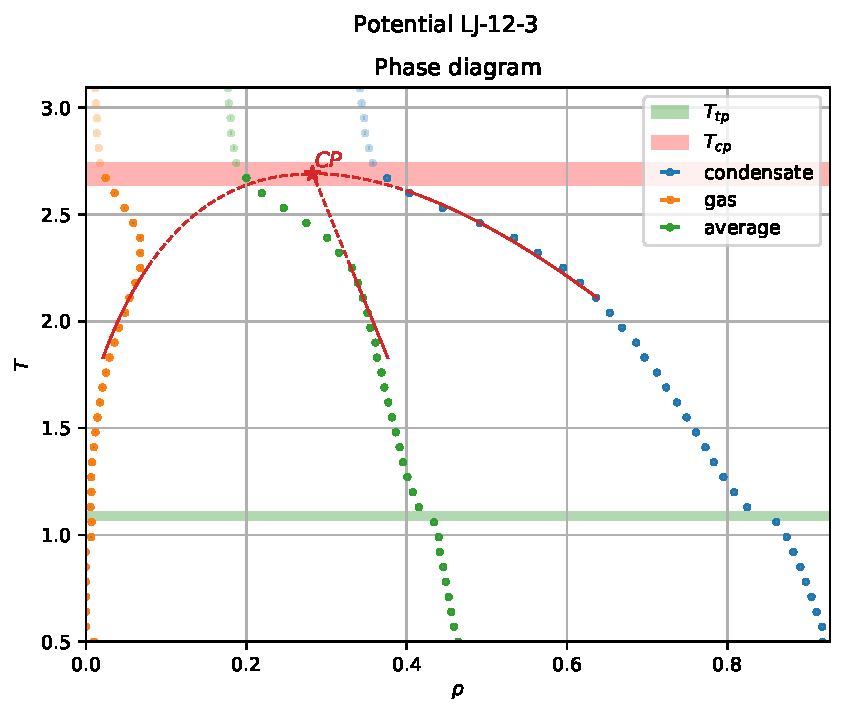
\includegraphics[width=\textwidth, keepaspectratio]{plot_phase_diagram_Potential LJ-12-3_1}
\end{minipage}
%\hfill
\begin{minipage}[h]{0.47\linewidth}
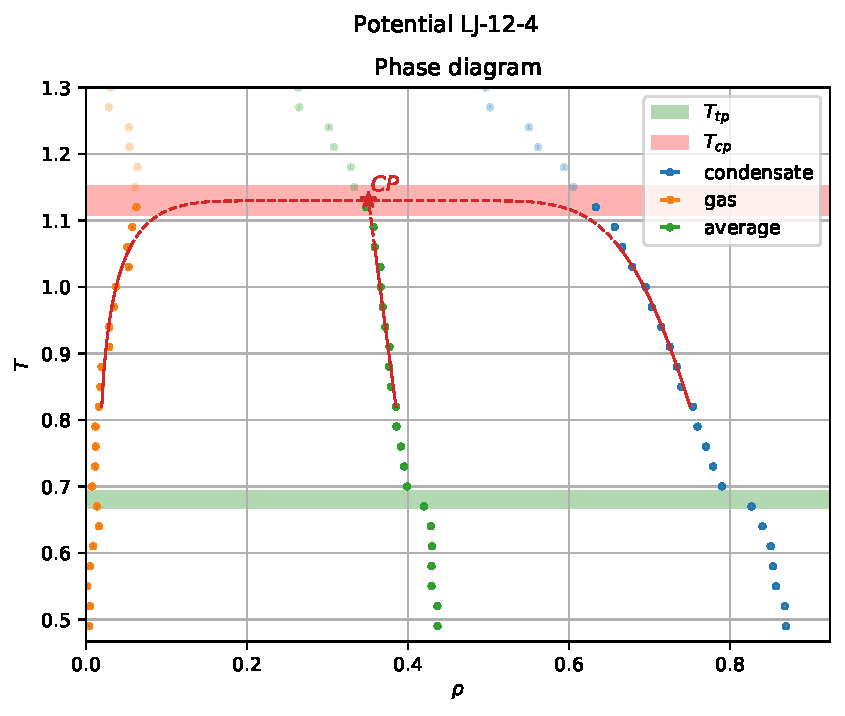
\includegraphics[width=\textwidth, keepaspectratio]{plot_phase_diagram_Potential LJ-12-4_1}
\end{minipage}

\begin{minipage}[h]{0.47\linewidth}
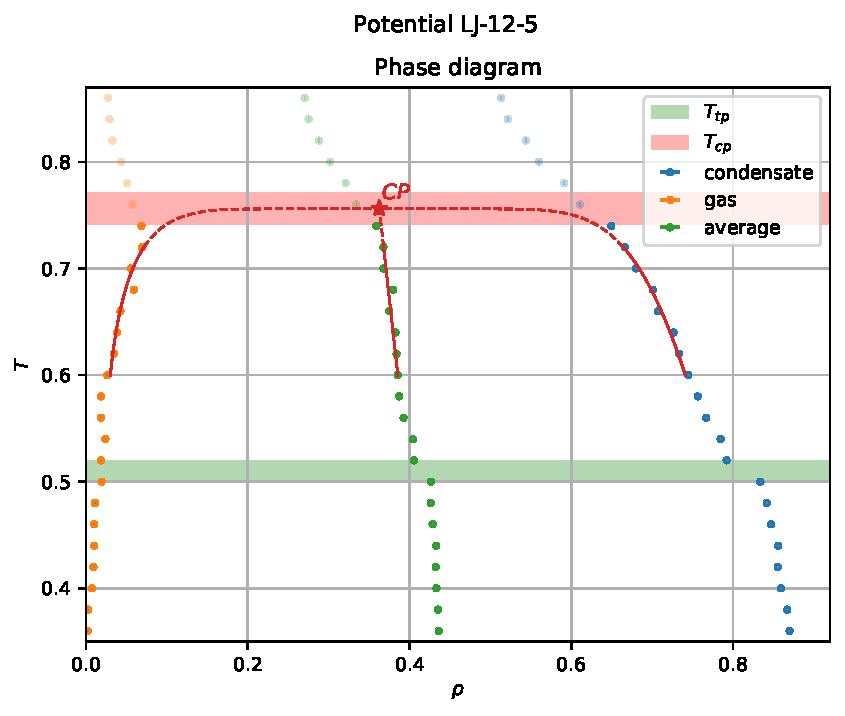
\includegraphics[width=\textwidth, keepaspectratio]{plot_phase_diagram_Potential LJ-12-5_1}
\end{minipage}
%\hfill
\begin{minipage}[h]{0.47\linewidth}
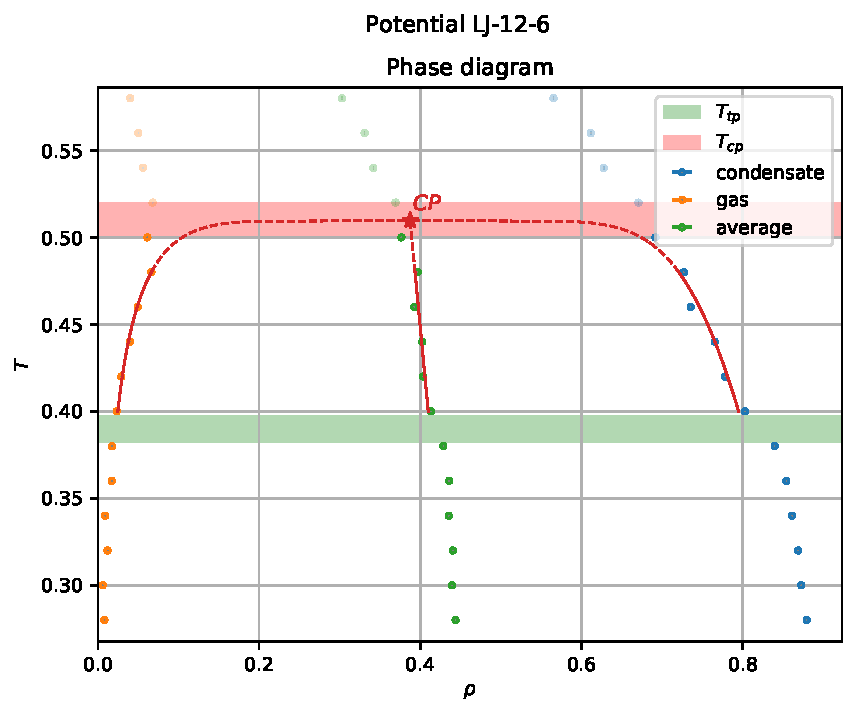
\includegraphics[width=\textwidth, keepaspectratio]{plot_phase_diagram_Potential LJ-12-6_1}
\end{minipage}
\label{risPhaseDiagrammExp}
\end{center}
\end{figure}

\end{column}

\begin{column}{0.5\linewidth}
\tiny{
\begin{equation}
\begin{aligned}
\rho_l - \rho_g &\simeq A (T_{CP} - T)^{\beta_c} \\
\frac{\rho_l + \rho_g}{2} &\simeq \rho_{CP} + a(T_{CP} - T)
\end{aligned}
\label{eqFitFhase}
\end{equation}
где $T_{CP}, \rho_{CP}$ - эффективная температура и плотность критической точки, $A, a$ - варьируемые параметры, $\rho_l, \rho_g$ - плотность жидкости и газа соответственно, $\beta_c$ - критический индекс системы.
}

\tiny{
\begin{table}[h]
%\begin{center}
\begin{tabular}{| l | l | l | l | l |}
\hline
    & $T_{TP}$  & $T_{CP}$  & $\rho_{CP}$   \\ \hline
LJ12-3  & 1.09  &  2.69   &  0.26   \\ \hline
LJ12-4  & 0.68  & 1.13    & 0.35    \\ \hline
LJ12-5  & 0.51  &  0.76   &  0.36   \\ \hline
LJ12-6  & 0.40  &  0.51   &  0.39   \\ \hline
\end{tabular}
%\end{center}
\caption{\tiny Параметры фазовых диаграмм для различных потенциалов взаимодействия. $T_{CP}$ - критическая температура, $\rho_{CP}$ - критическая плотность системы, $T_{TP}$ - температура тройной точки.}
\label{tablSystemConst}
\end{table}
}

\end{column}

\end{columns}
\vspace{2mm}
\tiny{
Kryuchkov N. P. et al. Phase diagram of two-dimensional colloids with Yukawa repulsion and dipolar attraction //The Journal of chemical physics. – 2019. – Т. 150. – №. 10. – С. 104903.
}
\end{frame}




\subsection{Анализ гистограмм распределения плотностей}


\begin{frame}
\transdissolve[duration=0.2]
\frametitle{Анализ гистограмм распределения плотностей}

\begin{columns}

\begin{column}{0.45\linewidth}
\tiny{
Равновесные колебания вблизи среднего значения объема определяются уравнением состояния системы, и соответствующая функция распределения вероятности $p(V)$ равна:
\begin{equation}
p(V) \varpropto \exp\left[ \frac{1}{2T} \left( \frac{\partial P}{\partial V} \right)  \left(V - V_0 \right)^2 \right],
\label{eqPv}
\end{equation}
где $P$ - давление, $V_0$ - максимум распределения объема, $V$ - объем.

Сделав замену $V = 1 / \rho$, получим следующее уравнение для аппроксимации верхушки гистограмм:
\begin{equation}
\begin{aligned}
p(\rho) &\varpropto \exp \left[ - K \left(\rho_{max}- \rho \right)^2 \right] \\
K &= \frac{1}{2T\rho_{max}^2} \left( \frac{\partial P}{\partial \rho} \right)
\end{aligned}
\label{eqFitRho}
\end{equation}
где $\rho_{max}$ - плотность максимума распределения. Верно для систем с мягким взаимодействием. 
}
\end{column}


\begin{column}{0.55\linewidth}

\begin{figure}[h]
\center{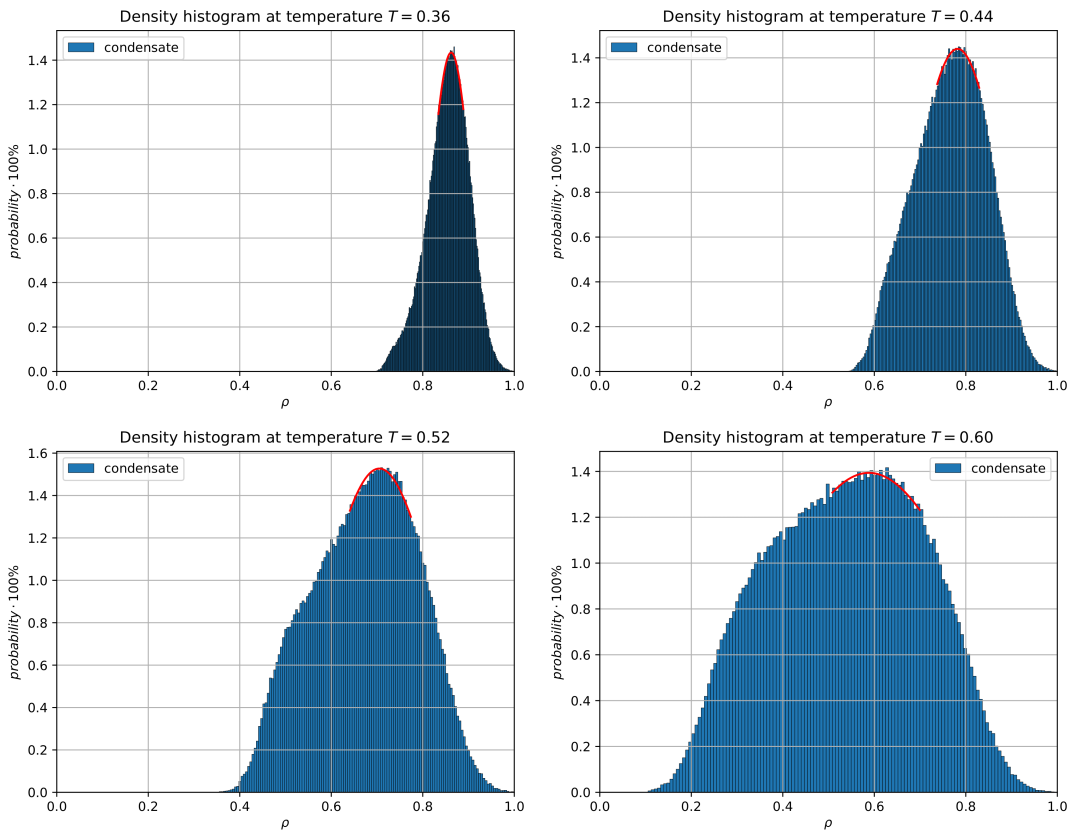
\includegraphics[width=\textwidth,  keepaspectratio]{FitDensity}}
\caption{\tiny Аппроксимация пика распределения плотности при различной
температуре на примере потенциала LJ12-6.}
\end{figure}

\end{column}

\end{columns}
\vspace{2mm}
\tiny{
Landau LD. EM Lifshitz Statistical Physics // Course of Theoretical
Physics. –– 1980. –– Vol. 5. –– P. 396–400.
}

\end{frame}





\begin{frame}
\transdissolve[duration=0.2]

\begin{columns}

\begin{column}{0.6\linewidth}

\begin{figure}[h]
\begin{center}
\begin{minipage}[h]{0.45\linewidth}
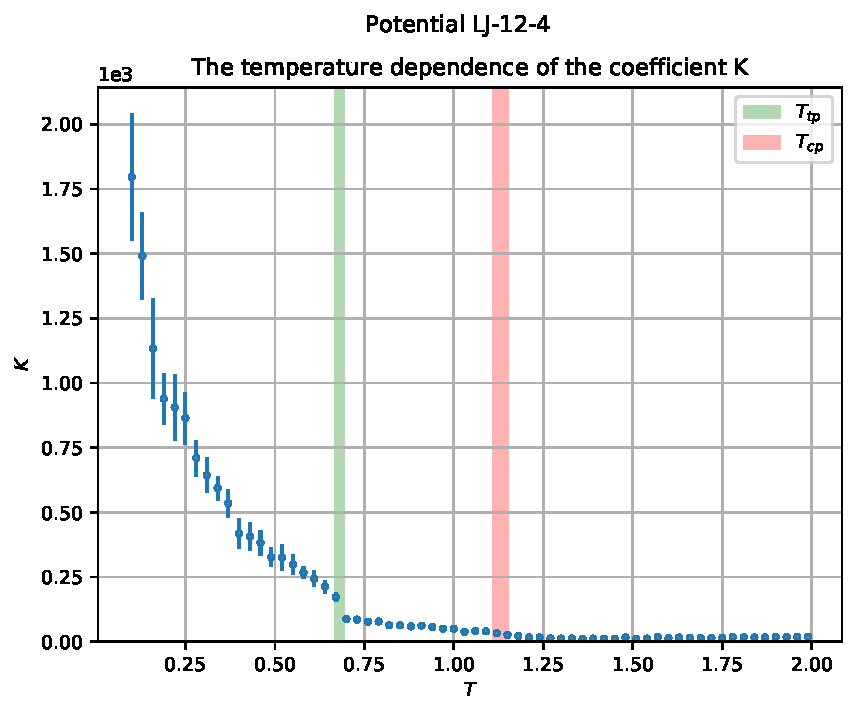
\includegraphics[width=\textwidth, keepaspectratio]{plot_K_Potential LJ-12-4_1}
\end{minipage}
%\hfill
\begin{minipage}[h]{0.45\linewidth}
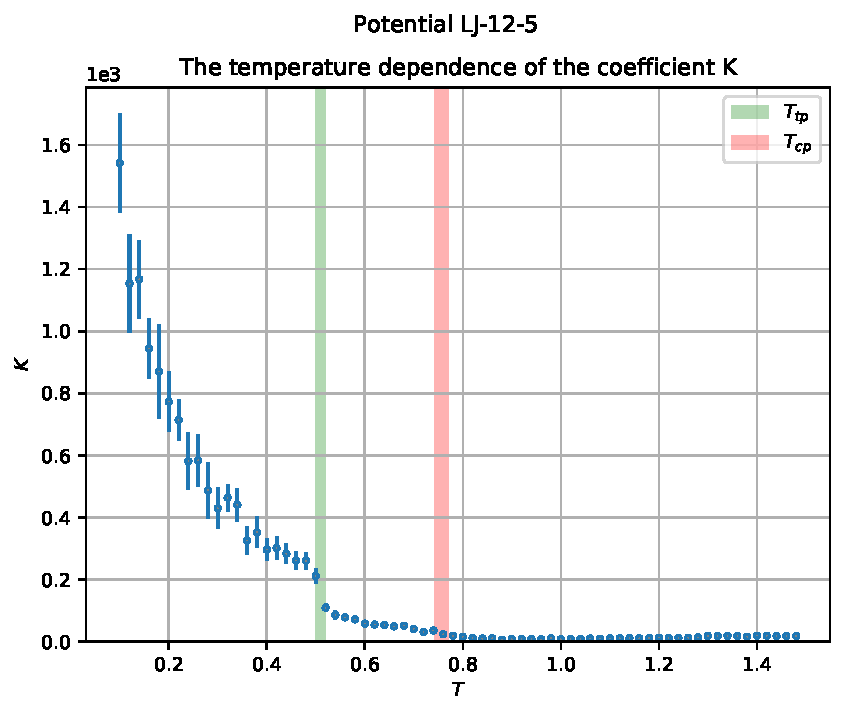
\includegraphics[width=\textwidth, keepaspectratio]{plot_K_Potential LJ-12-5_1}
\end{minipage}

\begin{minipage}[h]{0.45\linewidth}
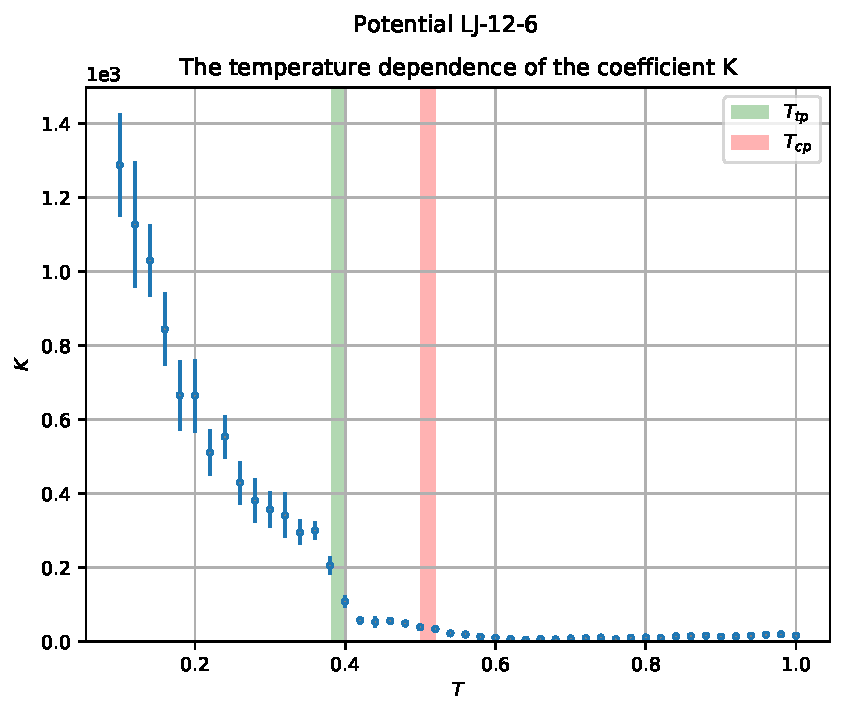
\includegraphics[width=\textwidth, keepaspectratio]{plot_K_Potential LJ-12-6_1}
\end{minipage}
%\hfill
\begin{minipage}[h]{0.45\linewidth}
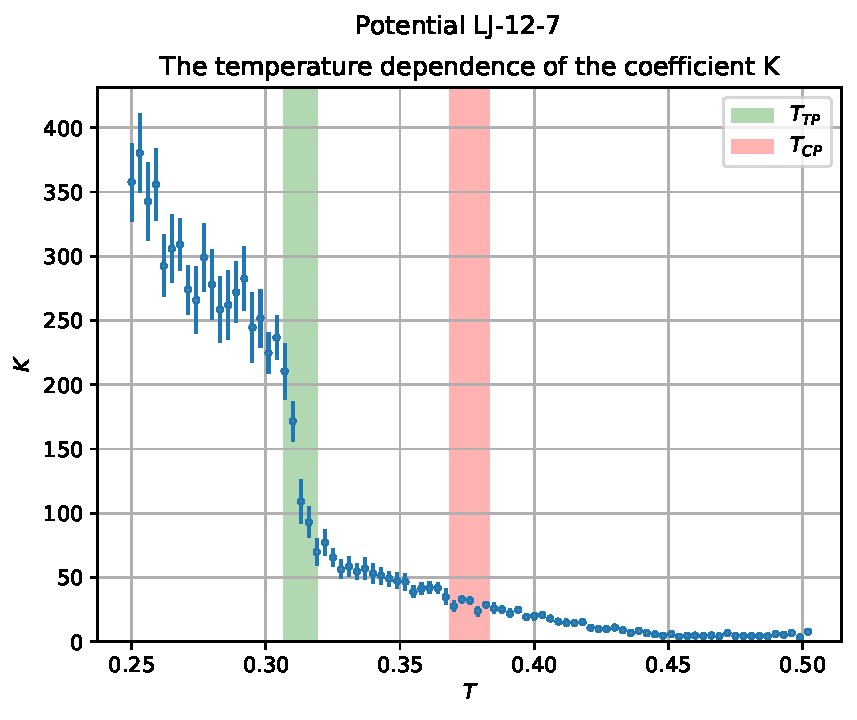
\includegraphics[width=\textwidth, keepaspectratio]{plot_K_Potential LJ-12-7_1}
\end{minipage}
\caption{\tiny Температурная зависимость коэффициента $K$.}
\label{risK}
\end{center}
\end{figure}

\end{column}

\begin{column}{0.45\linewidth}
\tiny{
По коэффициенту $K$ можно определить сжимаемость и адиабатическая скорость звука:
\begin{equation}
\begin{aligned}
\beta = \frac{1}{\rho_0} \frac{\partial \rho}{\partial P} \\
C = \sqrt{\frac{\partial P}{\partial \rho}},
\end{aligned}
\label{eqCBeta}
\end{equation}
где $\beta$ - сжимаемости, $C$ - скорость звука в веществе.

Выразив данные величины через коэффициент $K$, получим следующие формулы:
\begin{equation}
\begin{aligned}
\beta = \frac{1}{2T\rho_0\rho_{max}^2K}\\
C = \rho_{max}\sqrt{2TK}
\end{aligned}
\label{eqCBetaK}
\end{equation}
Верно для систем с мягким взаимодействием. 
}
\end{column}

\end{columns}
\end{frame}





\begin{frame}
\transdissolve[duration=0.2]

\begin{figure}[h]
\begin{center}
\begin{minipage}[h]{0.35\linewidth}
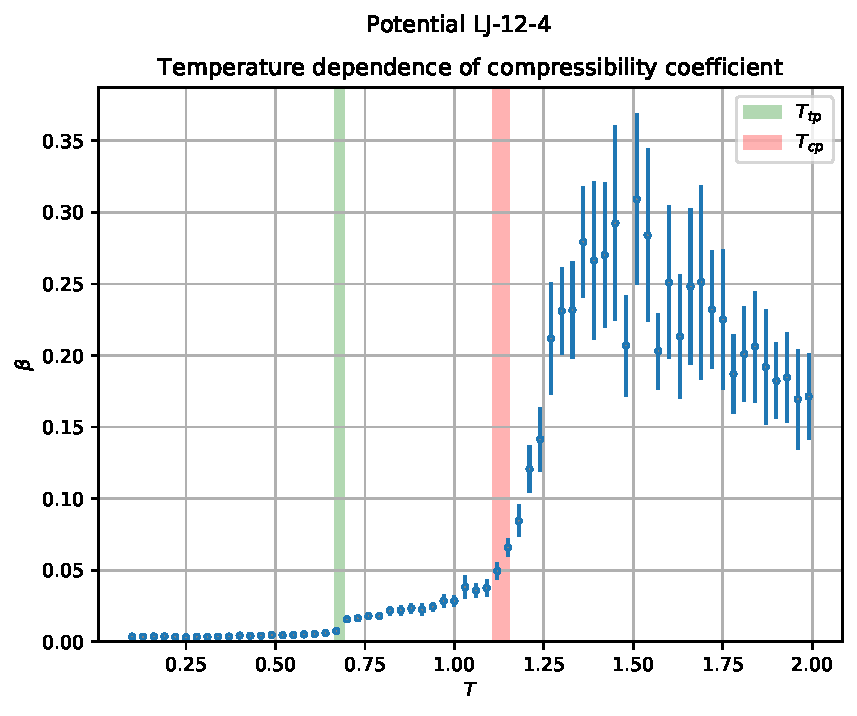
\includegraphics[width=\textwidth, keepaspectratio]{plot_compress_Potential LJ-12-4_1}
\end{minipage}
%\hfill
\begin{minipage}[h]{0.35\linewidth}
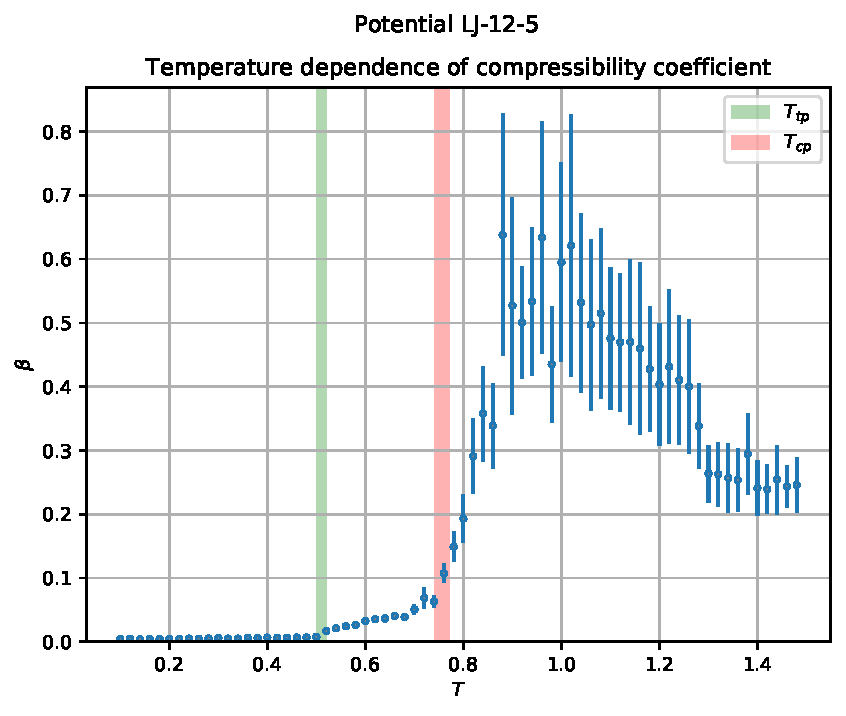
\includegraphics[width=\textwidth, keepaspectratio]{plot_compress_Potential LJ-12-5_1}
\end{minipage}

\begin{minipage}[h]{0.35\linewidth}
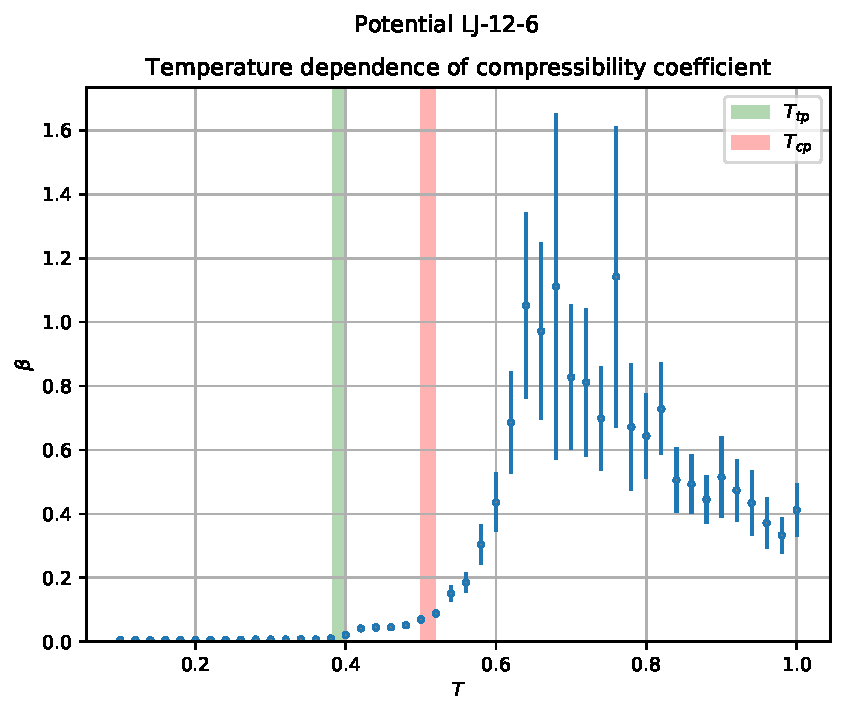
\includegraphics[width=\textwidth, keepaspectratio]{plot_compress_Potential LJ-12-6_1}
\end{minipage}
%\hfill
\begin{minipage}[h]{0.35\linewidth}
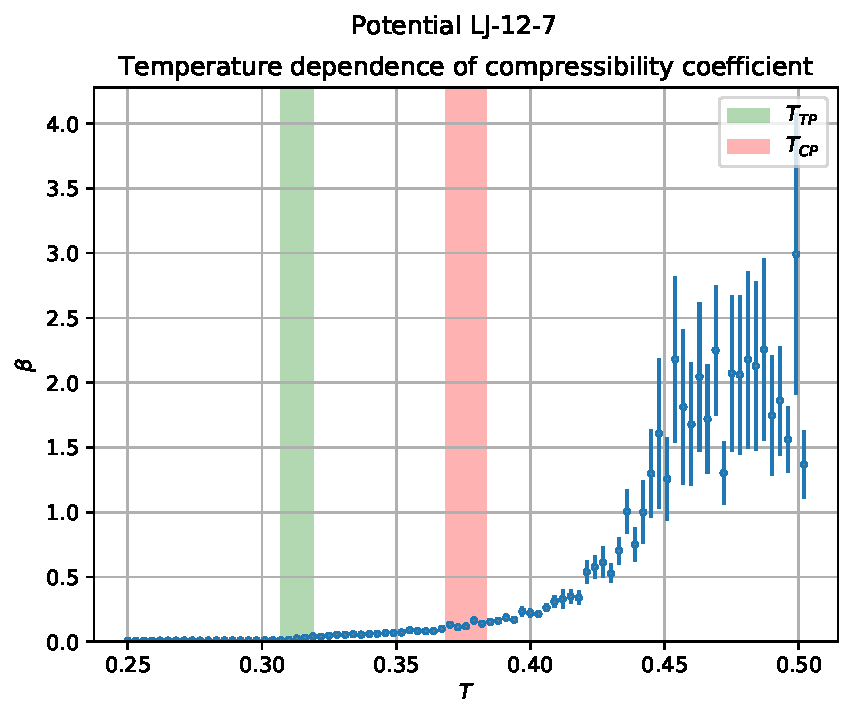
\includegraphics[width=\textwidth, keepaspectratio]{plot_compress_Potential LJ-12-7_1}
\end{minipage}
\caption{\tiny Температурная зависимость $\beta$, совпадающая с сжимаемостью в мягких взаимодействиях, при различных потенциалах.}
\label{risBeta}
\end{center}
\end{figure}

\end{frame}





\begin{frame}
\transdissolve[duration=0.2]

\begin{figure}[h]
\begin{center}
\begin{minipage}[h]{0.35\linewidth}
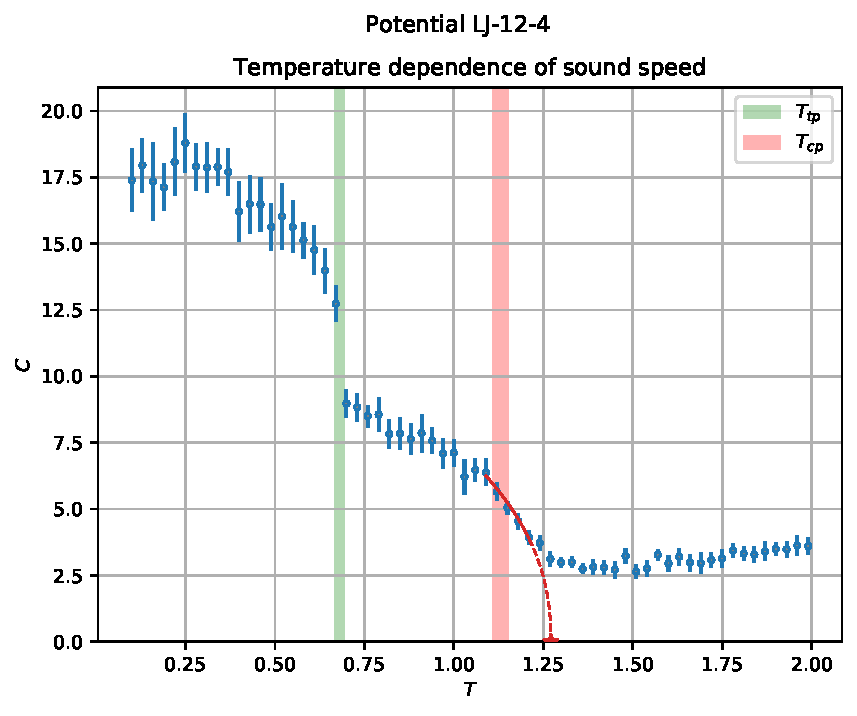
\includegraphics[width=\textwidth, keepaspectratio]{sound_speed_Potential LJ-12-4_1}
\end{minipage}
%\hfill
\begin{minipage}[h]{0.35\linewidth}
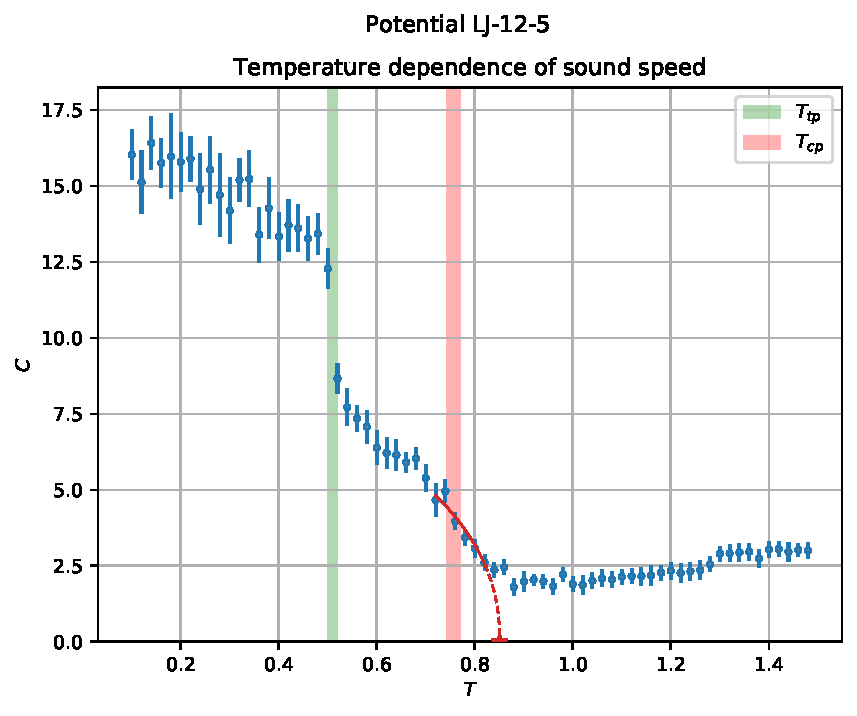
\includegraphics[width=\textwidth, keepaspectratio]{sound_speed_Potential LJ-12-5_1}
\end{minipage}

\begin{minipage}[h]{0.35\linewidth}
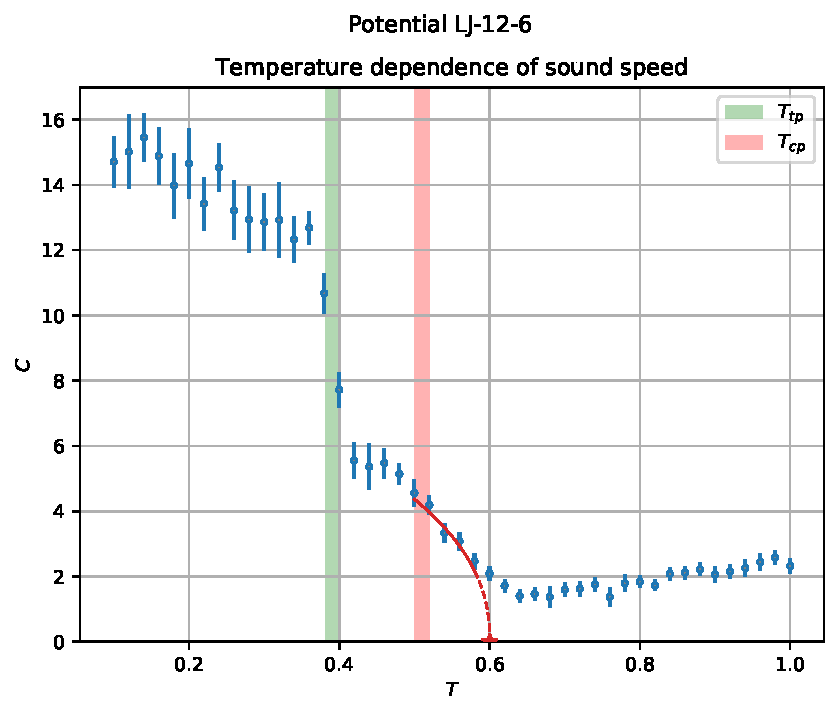
\includegraphics[width=\textwidth, keepaspectratio]{sound_speed_Potential LJ-12-6_1}
\end{minipage}
%\hfill
\begin{minipage}[h]{0.35\linewidth}
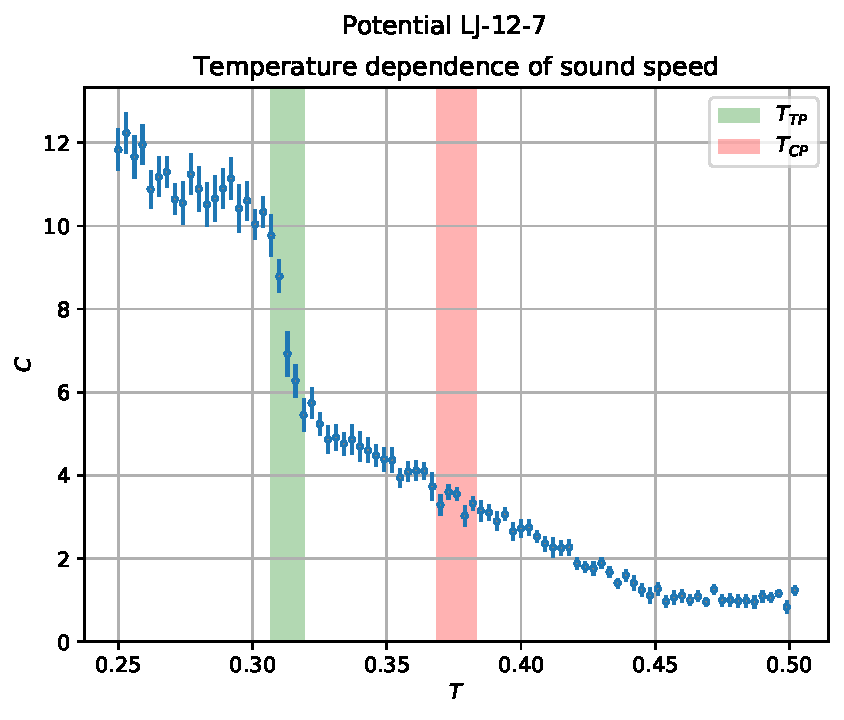
\includegraphics[width=\textwidth, keepaspectratio]{sound_speed_Potential LJ-12-7_1}
\end{minipage}
\caption{\tiny Температурная зависимость $C$, совпадающая со скоростью звука в мягких взаимодействиях, при различных потенциалах.}
\label{risC}
\end{center}
\end{figure}

\end{frame}





\begin{frame}
\transdissolve[duration=0.2]
\frametitle{Влияние дальнодействия притяжения}

\begin{figure}[h]
\begin{center}
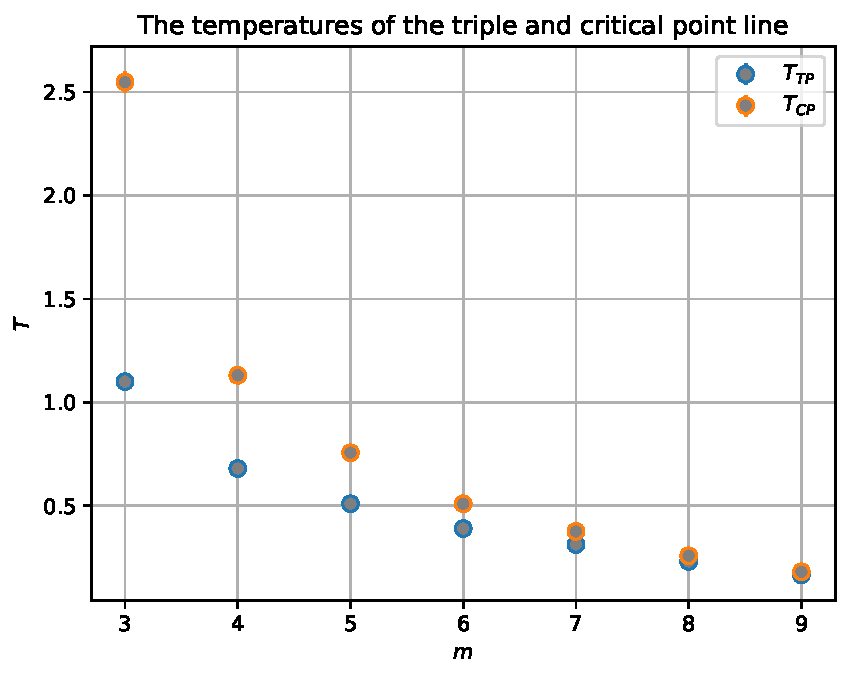
\includegraphics[width=0.7\textwidth]{temperatures_triple_critical_Widom}
\caption{ \tiny Температуры тройной и критической точки в зависимости от степени $m$.}
\label{risTcpTtp}
\end{center}
\end{figure}

\end{frame}





\begin{frame}
\transdissolve[duration=0.2]
\frametitle{Влияние дальнодействия притяжения на фазовую диаграмму}

\begin{figure}[h]
\begin{center}
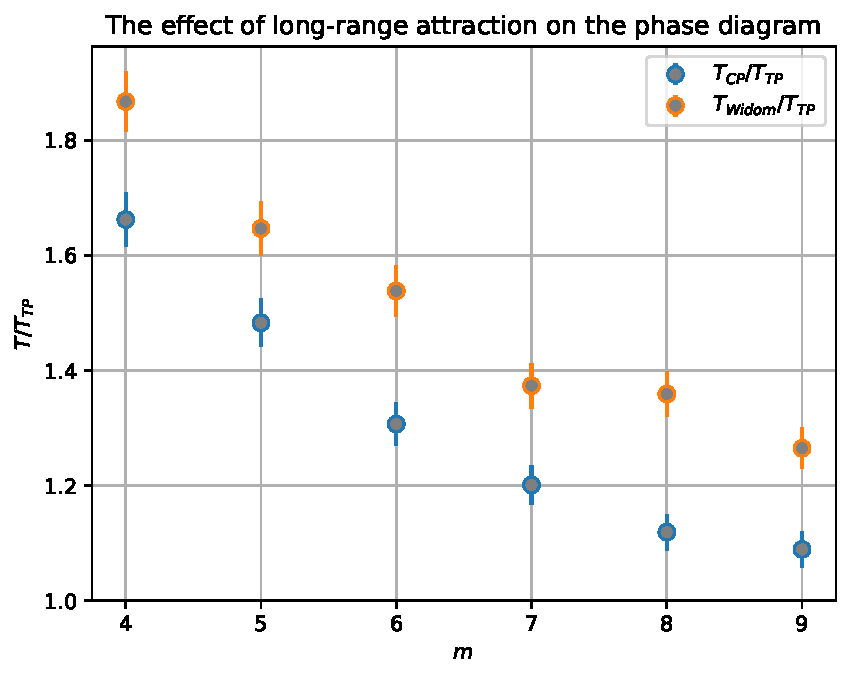
\includegraphics[width=0.7\textwidth]{effect_of_long-range_attraction}
\caption{\tiny Отношение температур критической точки к тройной в зависимости от степени $m$.}
\label{risTcpTtpWidoml}
\end{center}
\end{figure}

\end{frame}




%\section{Изучение диффузии}
\subsection{ }


\begin{frame}
\begin{center}
\vspace{5mm}
\textbf{<<ДИФФУЗИЯ ОТ ТРОЙНОЙ ДО \\ КРИТИЧЕСКОЙ ТОЧКИ>>}
\end{center}
\end{frame}


\subsection{Вычисление параметров переноса}




\begin{frame}
\transdissolve[duration=0.2]
\frametitle{Вычисление коэффициента диффузии методами МД}

\begin{columns}

\begin{column}{0.5\linewidth}

\begin{figure}[h]
\begin{center}
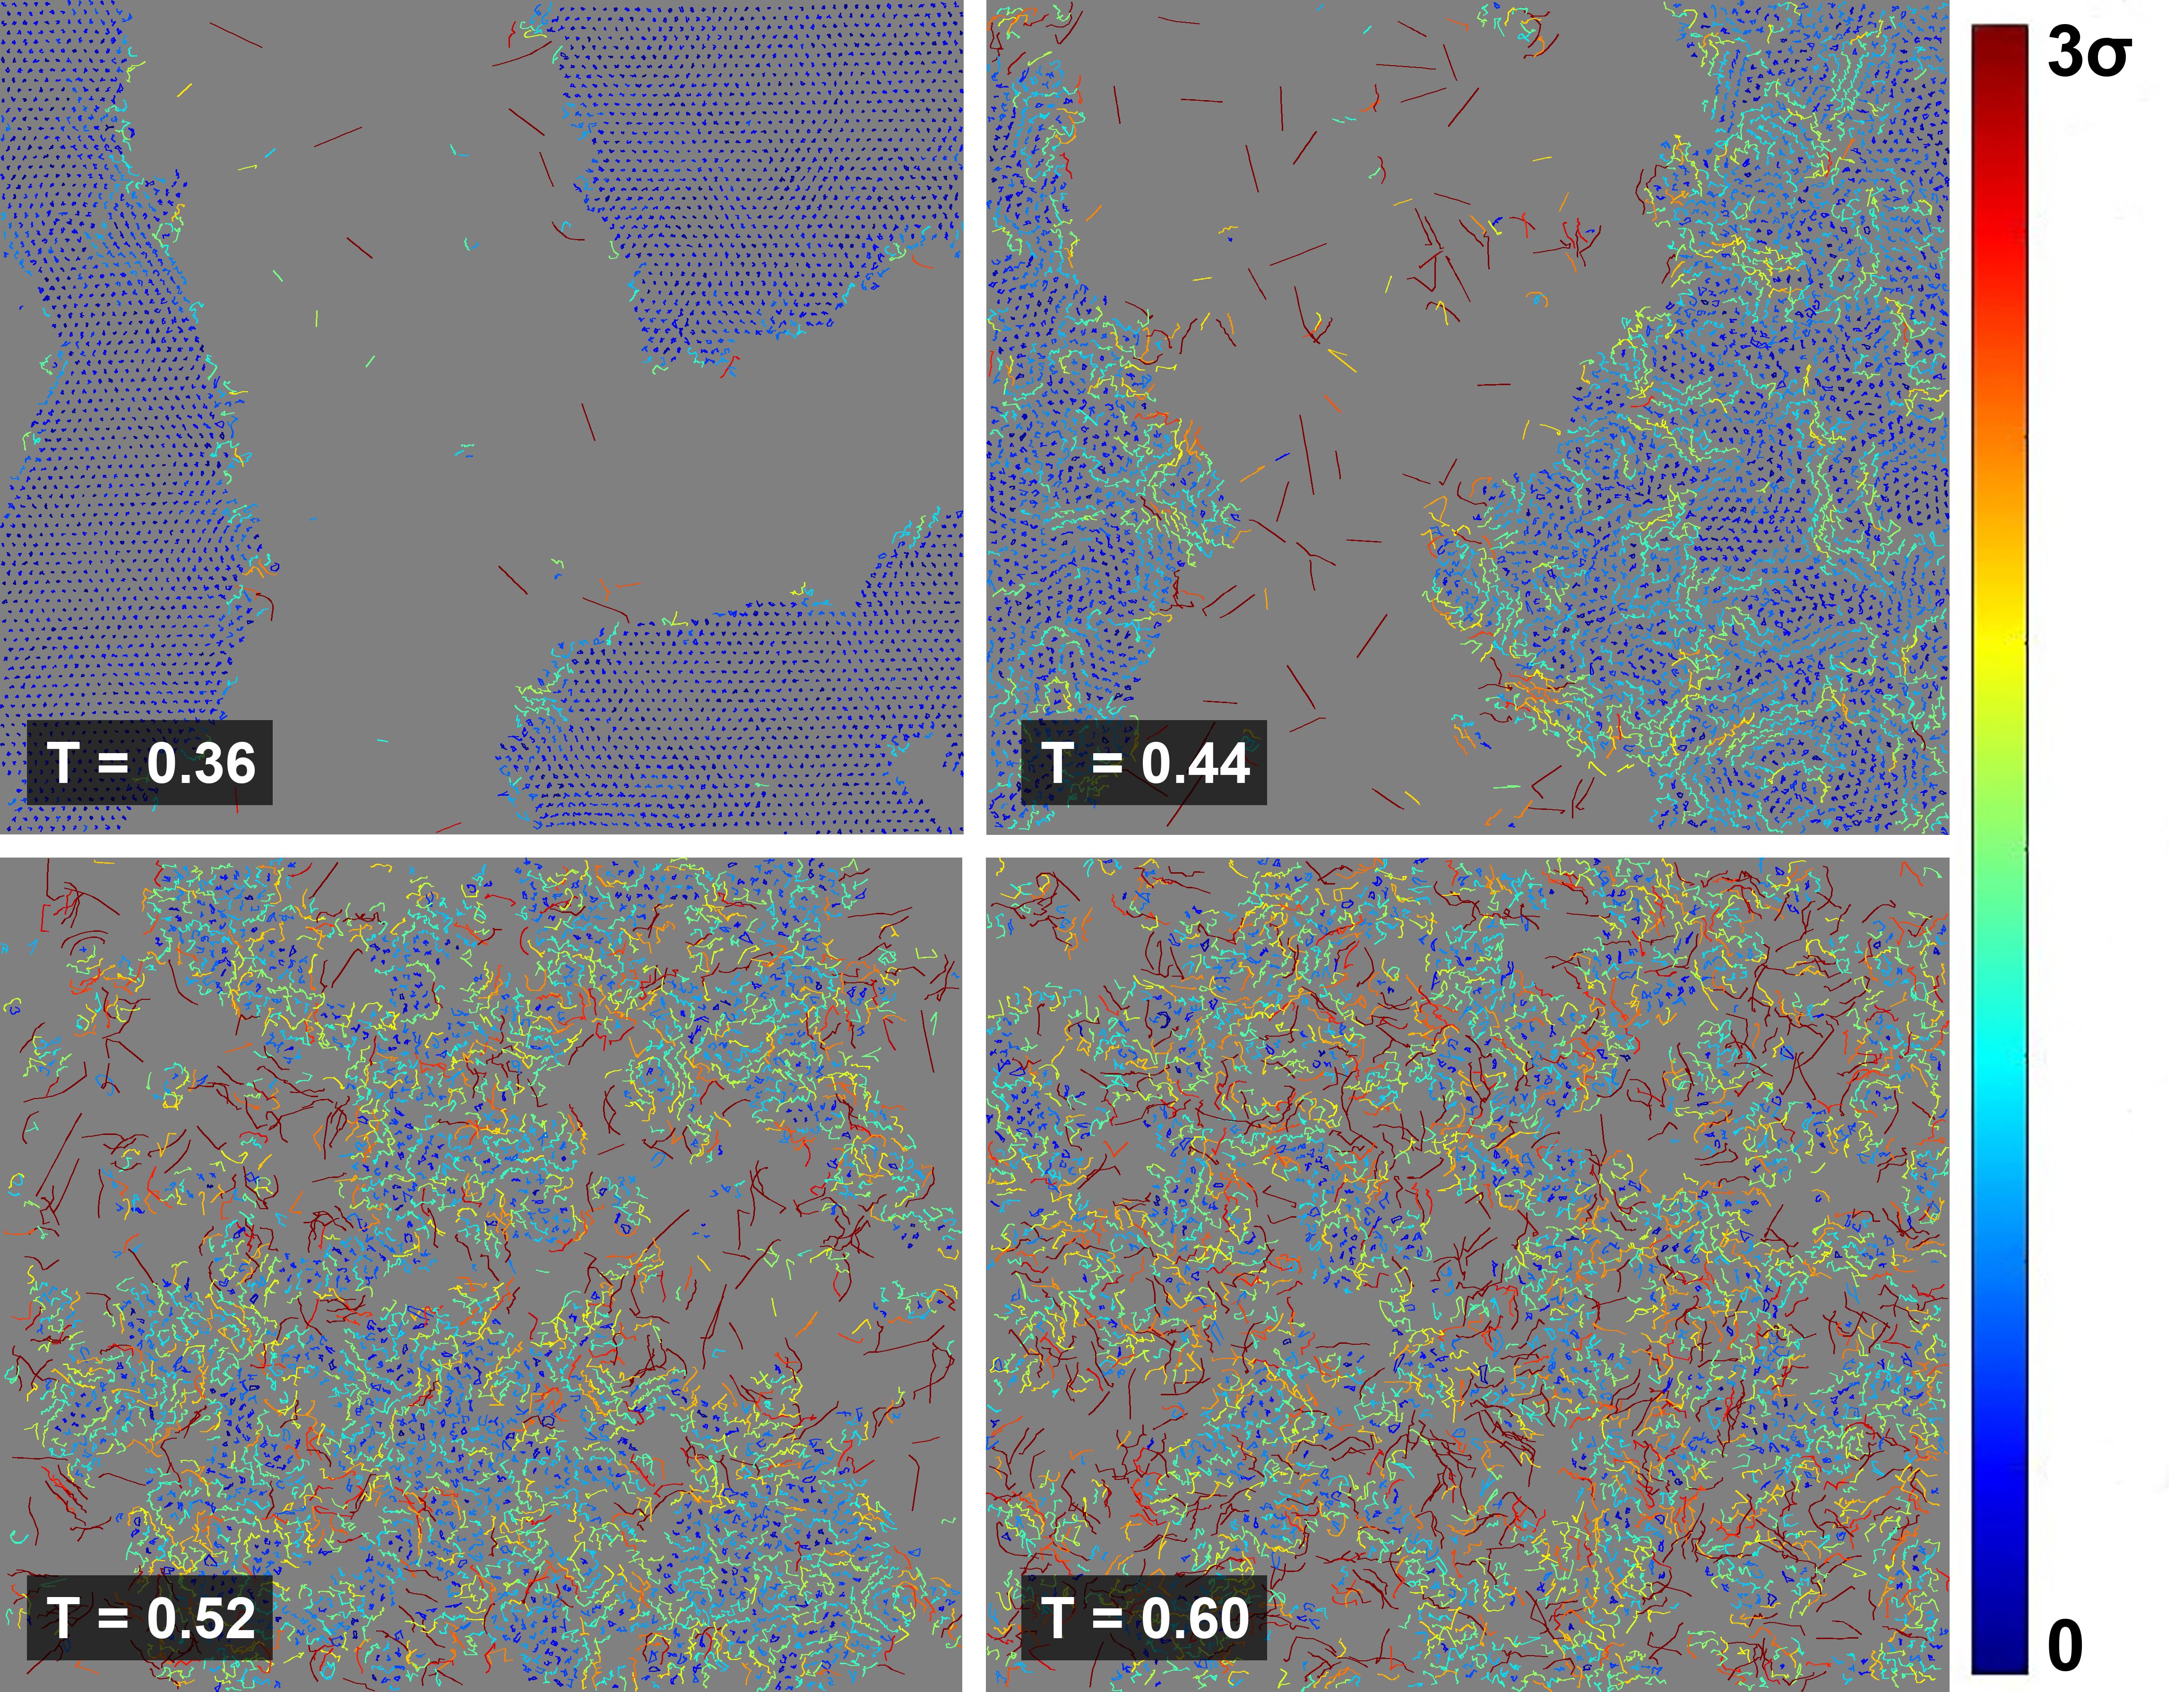
\includegraphics[width=\textwidth]{Diffusion}
\caption{\tiny Смещение частиц от начального положения за 10 кадров моделирования. Цветом показана величина смещения в $\sigma$ (единица измерения длинны).}
\label{risTreck}
\end{center}
\end{figure}

\end{column}
\begin{column}{0.5\linewidth}
\tiny{

Зная смещения всех частиц от их изначального положения в системе, с $t = 0$, можно рассчитать среднеквадратичное смещение частиц с помощью уравнения:
\begin{equation}
    \sigma^2(t) = \sum\limits_{\alpha = 1}^{N(t)} (r_{\alpha}(t) - r_{\alpha}(0))^2 / N(t),
    \label{eqRMS}
\end{equation}
где $\sigma^2(t)$ - среднеквадратичное смещение частиц, $N(t)$ - количество частиц в данный момент времени в кадре, $r_{\alpha}(t)$ - положение частицы в момент времени $t$, $r_{\alpha}(0)$ - положение частицы в начальный момент времени $t = 0$.

}
\end{column}

\end{columns}
\end{frame}





\begin{frame}
\transdissolve[duration=0.2]
\frametitle{Вычисление коэффициента диффузии методами МД}

\begin{columns}

\begin{column}{0.55\linewidth}

\begin{figure}[h]
\begin{center}
\begin{minipage}[h]{0.45\linewidth}
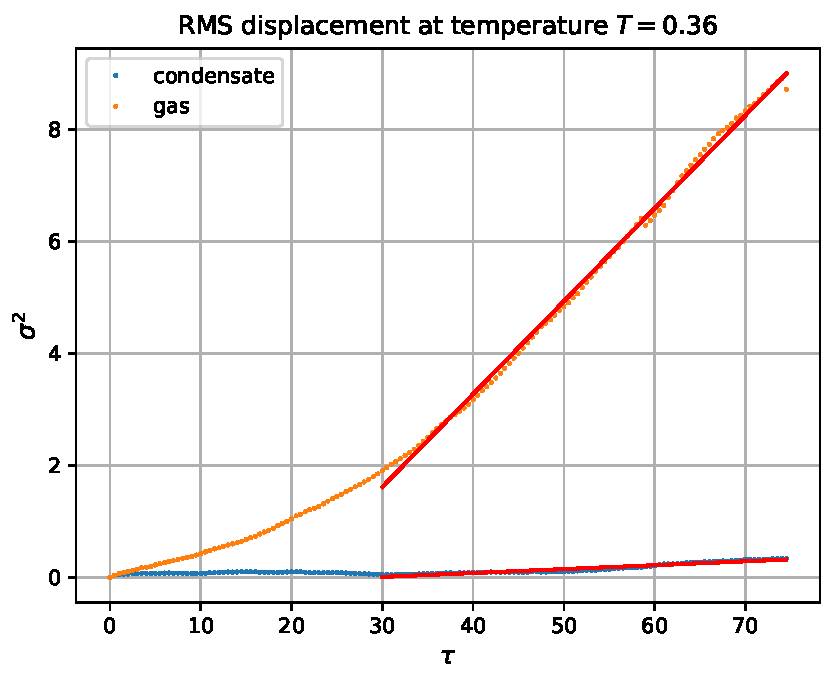
\includegraphics[width=\textwidth, keepaspectratio]{diffusion_fit_0.36}
\end{minipage}
%\hfill
\begin{minipage}[h]{0.45\linewidth}
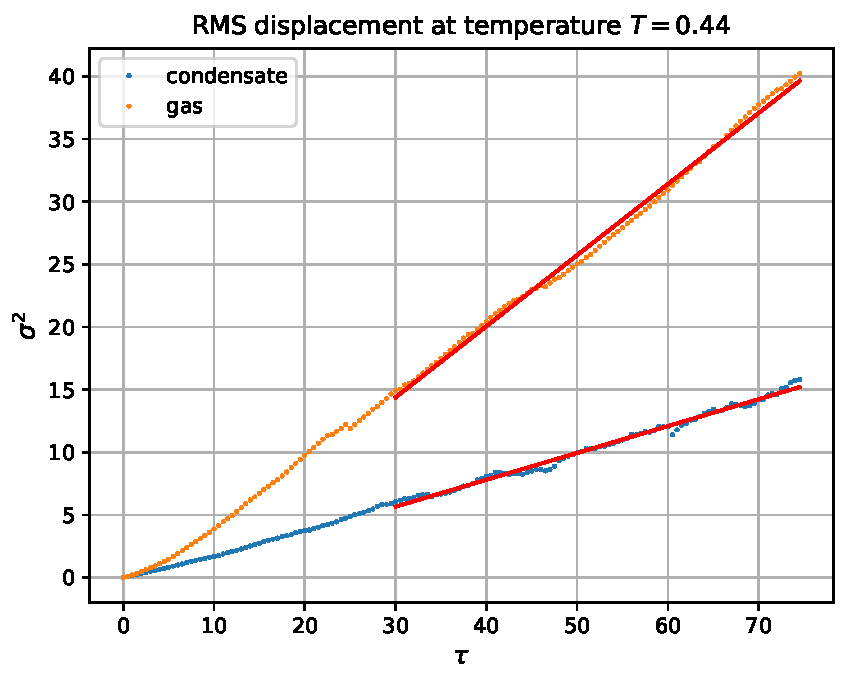
\includegraphics[width=\textwidth, keepaspectratio]{diffusion_fit_0.44}
\end{minipage}

\begin{minipage}[h]{0.45\linewidth}
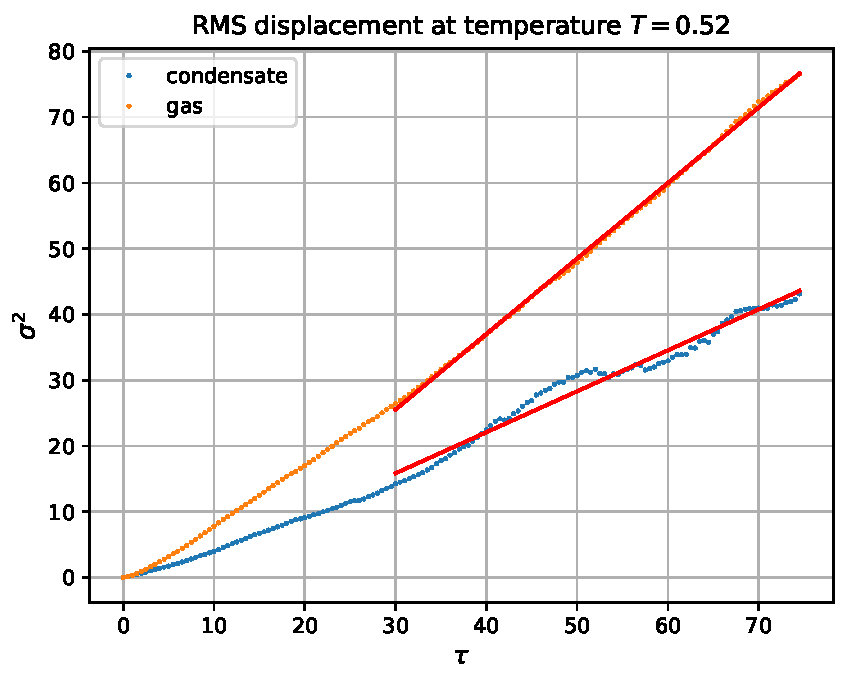
\includegraphics[width=\textwidth, keepaspectratio]{diffusion_fit_0.52}
\end{minipage}
%\hfill
\begin{minipage}[h]{0.45\linewidth}
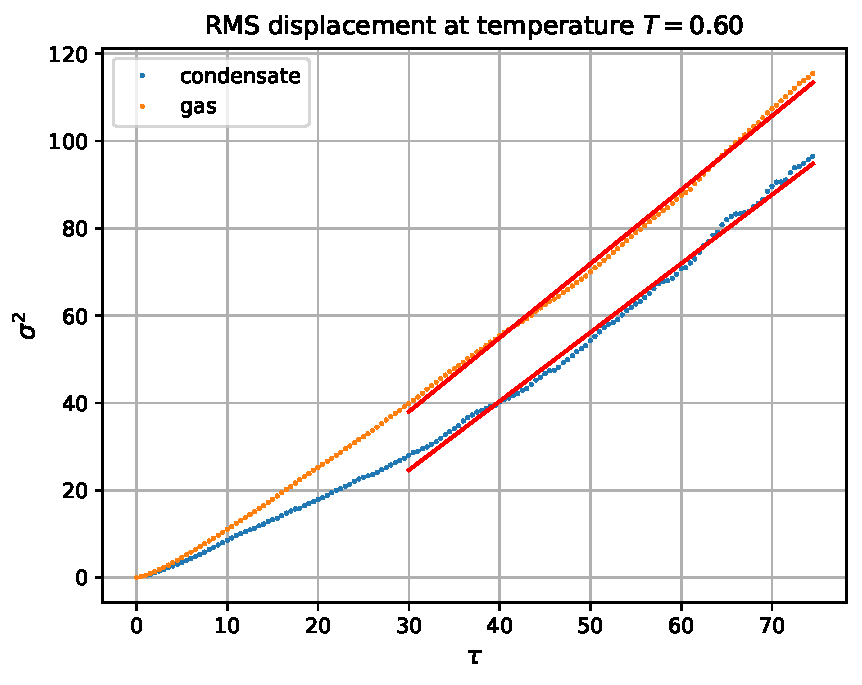
\includegraphics[width=\textwidth, keepaspectratio]{diffusion_fit_0.60}
\end{minipage}
\caption{\tiny Временная зависимость среднеквадратичного смещения частиц для различных температур на примере потенциала Леннарда-Джонса.}
\label{risRMS}
\end{center}
\end{figure}

\end{column}
\begin{column}{0.45\linewidth}
\tiny{

Так как для двумерной системы верно равенство $\sigma^2(t) = 4Dt$, то коэффициент диффузии выражается следующей формулой:
\begin{equation}
    D = \frac{\sigma^2(t)}{4t},
    \label{eqD}
\end{equation}
где $D$ - коэффициент диффузии в веществе.

Его можно получить путем аппроксимации среднеквадратичного смещения функцией $\sigma^2(t) = 4Dt + a$, где $a$ - подгоночный коэффициент.

Кроме диффузии можно вычислить подвижность частиц в системе, которая определяется следующим уравнением:
\begin{equation}
    \mu  = \frac{D}{T},
    \label{eqMuDiff}
\end{equation}
где $\mu$ - подвижность частиц.
}
\end{column}


\end{columns}
\end{frame}


%\section{Результаты Главы 3}
\subsection{Температурная зависимость диффузии и подвижности}


\begin{frame}
\transdissolve[duration=0.2]

\begin{figure}[h]
\begin{center}
\begin{minipage}[h]{0.35\linewidth}
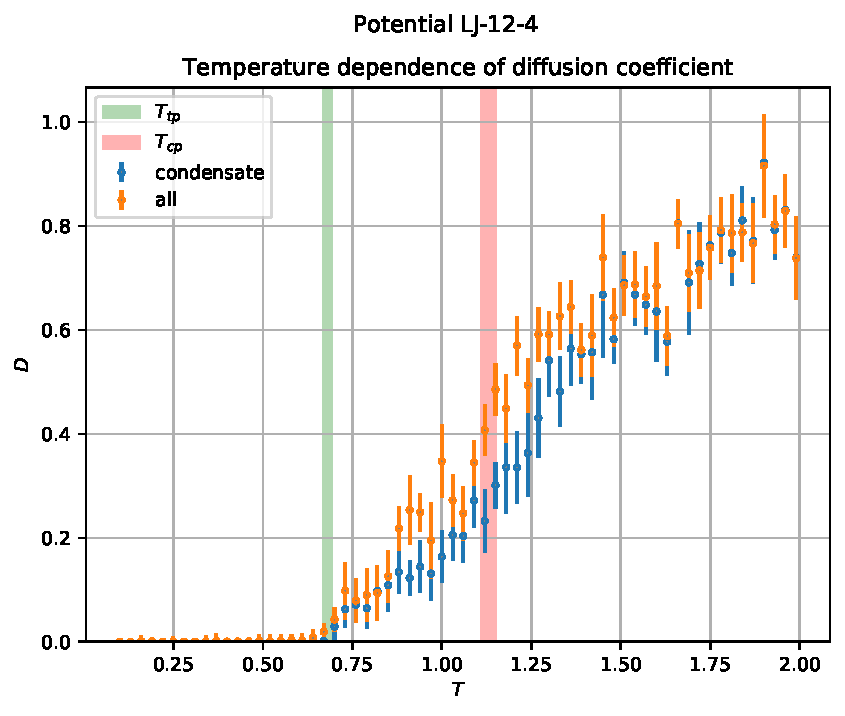
\includegraphics[width=\textwidth, keepaspectratio]{plot_diffusion_Potential LJ-12-4_1}
\end{minipage}
\begin{minipage}[h]{0.35\linewidth}
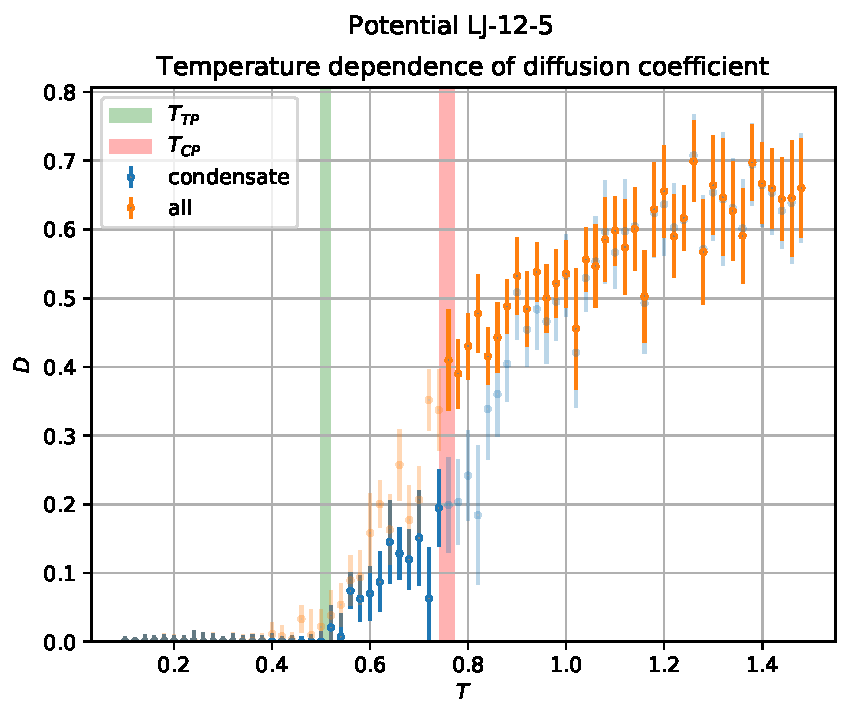
\includegraphics[width=\textwidth, keepaspectratio]{plot_diffusion_Potential LJ-12-5_1}
\end{minipage}
\begin{minipage}[h]{0.35\linewidth}
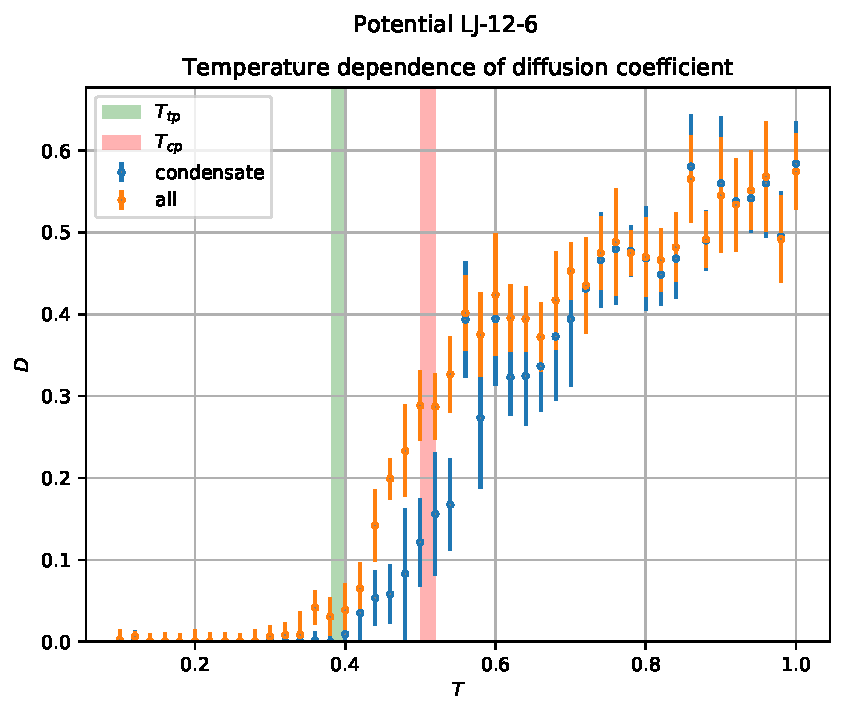
\includegraphics[width=\textwidth, keepaspectratio]{plot_diffusion_Potential LJ-12-6_1}
\end{minipage}
\begin{minipage}[h]{0.35\linewidth}
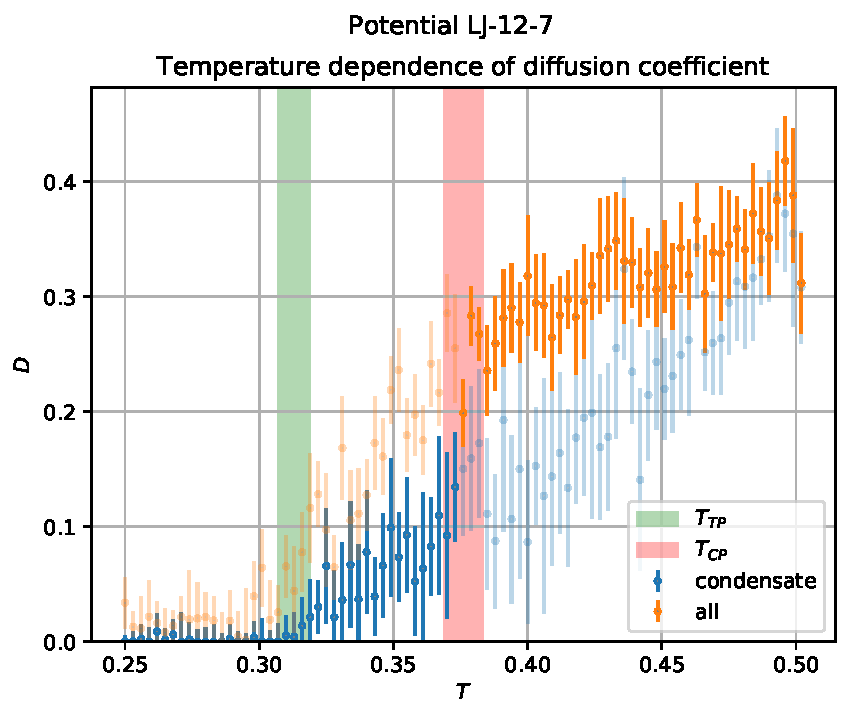
\includegraphics[width=\textwidth, keepaspectratio]{plot_diffusion_Potential LJ-12-7_1}
\end{minipage}
\caption{\tiny Температурная зависимость коэффициента диффузии для различных потенциалов взаимодействия.}
\label{risD}
\end{center}
\end{figure}

\end{frame}




\begin{frame}
\transdissolve[duration=0.2]

\begin{figure}[h]
\begin{center}
\begin{minipage}[h]{0.35\linewidth}
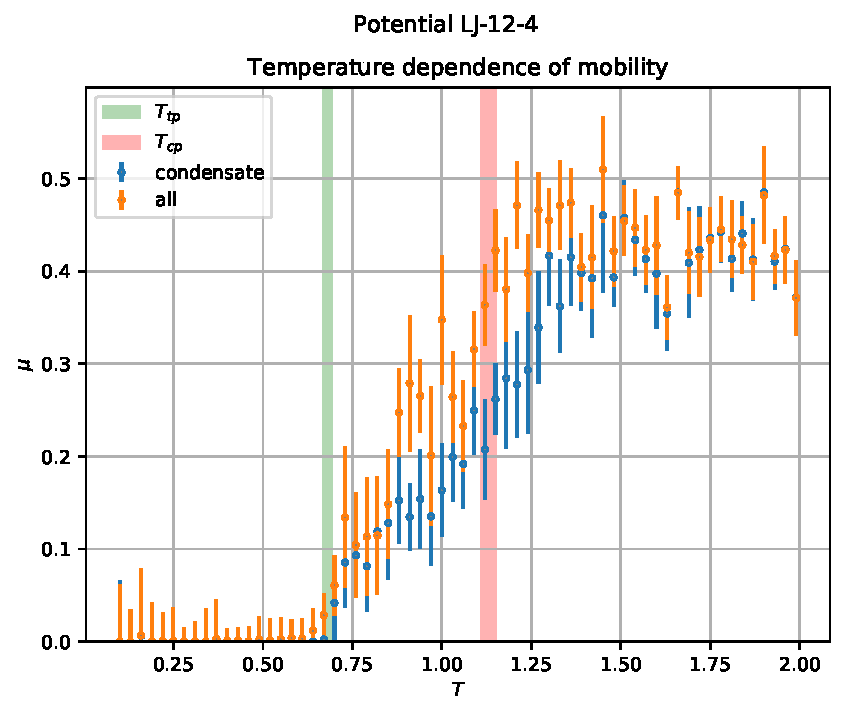
\includegraphics[width=\textwidth, keepaspectratio]{plot_mobility_Potential LJ-12-4_1}
\end{minipage}
%\hfill
\begin{minipage}[h]{0.35\linewidth}
\includegraphics[width=\textwidth, keepaspectratio]{plot_mobility_Potential LJ-12-5_1}
\end{minipage}
\begin{minipage}[h]{0.35\linewidth}
\includegraphics[width=\textwidth, keepaspectratio]{plot_mobility_Potential LJ-12-6_1}
\end{minipage}
%\hfill
\begin{minipage}[h]{0.35\linewidth}
\includegraphics[width=\textwidth, keepaspectratio]{plot_mobility_Potential LJ-12-7_1}
\end{minipage}
\caption{\tiny Температурная зависимость подвижности для различных потенциалов взаимодействия.}
\label{risMuDiff}
\end{center}
\end{figure}

\end{frame}







\begin{frame}
\transdissolve[duration=0.2]
\frametitle{Влияние дальнодействия притяжения на подвижность частиц}

\begin{figure}[h]
\begin{center}
\includegraphics[width=0.65\textwidth]{mobility_fitting_factors}
\caption{\tiny График зависимости параметров аппроксимации подвижности от тройной до критической точки линейной функцией.}
\label{risFittingFactors}
\end{center}
\end{figure}

\end{frame}





\subsection{Итоги ВКР}


\begin{frame}
	\transdissolve[duration=0.2]
	\frametitle{Основные результаты работы:}
	\footnotesize{
\begin{enumerate}
    \item В работе продемонстрированная актуальность метода изучения молекулярных систем с использованием построения диаграммы Вороного, который, используя только координаты частиц в разные моменты времени, позволяет узнать некоторые термодинамические параметры и параметры переноса в веществе.
    \item Проведена модернизация алгоритма классификации частиц на фазы, которая позволяет улучшить качество классификации и убрать артефакты из статистики распределения плотности частиц.
    \item Проведены серии моделирований обобщенного потенциала взаимодействия Леннарда--Джонса с различным дальнодействием притяжения для определения его роли в расположении критических и тройных точек на фазовых диаграммах вещества. 
    \item Реализован программный пакет для изучения диффузии с разрешением отдельных частиц, и с его помощью установлена роль дальнодействия притяжения на подвижность в веществе. 
\end{enumerate}
	}
\end{frame}


\begin{frame}
	\transdissolve[duration=0.2]
	\frametitle{Научная новизна:}
	\footnotesize{
\begin{enumerate}
    \item Впервые показана зависимость критической и тройной точки от дальнодействия притяжения.
    %\item Применен метод разбиения на ячейки Вороного для нахождения линии Видома.
    \item Показано влияние дальнодействия притяжения потенциала на подвижность частиц в веществе. 
\end{enumerate}
	}
\end{frame}


%\begin{frame}
%	\transdissolve[duration=0.2]
%	\frametitle{Публикации}
%	\footnotesize{
%\begin{enumerate}
%    \item Публикация 1.
%    \item Публикация 2.
%\end{enumerate}
%	}
%\end{frame}



\subsection{ }


\begin{frame}
\center{\Huge Спасибо за внимание!}
\end{frame}


\end{document}